
\documentclass[a4paper]{article}
\usepackage{pslatex}
\usepackage[T1]{fontenc}
\usepackage[utf8x]{inputenc}
\setlength\parskip{\medskipamount}
\setlength\parindent{0pt}
\usepackage{graphicx}
\usepackage{amssymb}
%\usepackage{hyperref}

\makeatletter

\providecommand{\boldsymbol}[1]{\mbox{\boldmath $#1$}}
\newcommand{\ASL}			{ASL}
\newcommand{\OSC}[1]		{\texttt{#1}}
\newcommand{\lra}			{$\leftrightarrow$}
\newcommand{\seg}[1]		{Seg(#1)}

\setlength{\parskip}{1mm}

\makeatother

\begin{document}

\title{FaustLive - Control/Compute/Communicate \\ All The Possibilities\\ v.2.0}

\author{Grame, Centre National de Création Musicale\\
{\small <research@grame.fr>} \\
\vspace{2mm}
[ANR-12-CORD- 0009] and [ANR-13-BS02-0008]
}

\maketitle

\topskip0pt

\vspace{\fill}

\vspace{\fill}
%==================================================================================================
\newpage
\tableofcontents

\newpage
\section{The Control-Compute-Communicate Model}

RECOPIER CE QUI A DEJA ETE FAIT LA DESSUS

\newpage
\section{Remote}

\begin{itemize}
\item Implement remote control --> SON COTE ORDI
\item Implement publish feature --> SON COTE IPHONE
\item 
\end{itemize}

The main difficulty is to think through the interactions of every feature:\\
- local/remote factories \\
- remote control (OSC, HTTP, NetJack) \\
And make sure we have the exact same behavior when local or remote, etc \\

For now, it is possible to use the remote processing or the publish feature but it was never validated that every thing works together. \\


--> Publish/Remote/Drop pour créer des factory : peut-être faire des composants différenciés \\
--> DNS dans le but de creéer une interface OSC/HTTP ou autre \\

--> Faire peut-être une spécification des fonctionnalités remote qu'on voudrait en essayant de spécifier les différentes briques à désimbriquer... \\

\section{Remote All the use cases and Configurations}

\subsection{Configurations}
To describe all the possible configurations, we use the "Control-Compute-Communicate" description. 

%%%%%%%%%%%%%%MAIN CONFIG%%%%%%%%%%%%%%%%%
\newpage
\subsection{FaustLive Main Use}
This is the usual configuration for any Faust application, whether it is a standalone application, a plugin or running in FaustLive.
\begin{figure}[!h]
\begin{center}
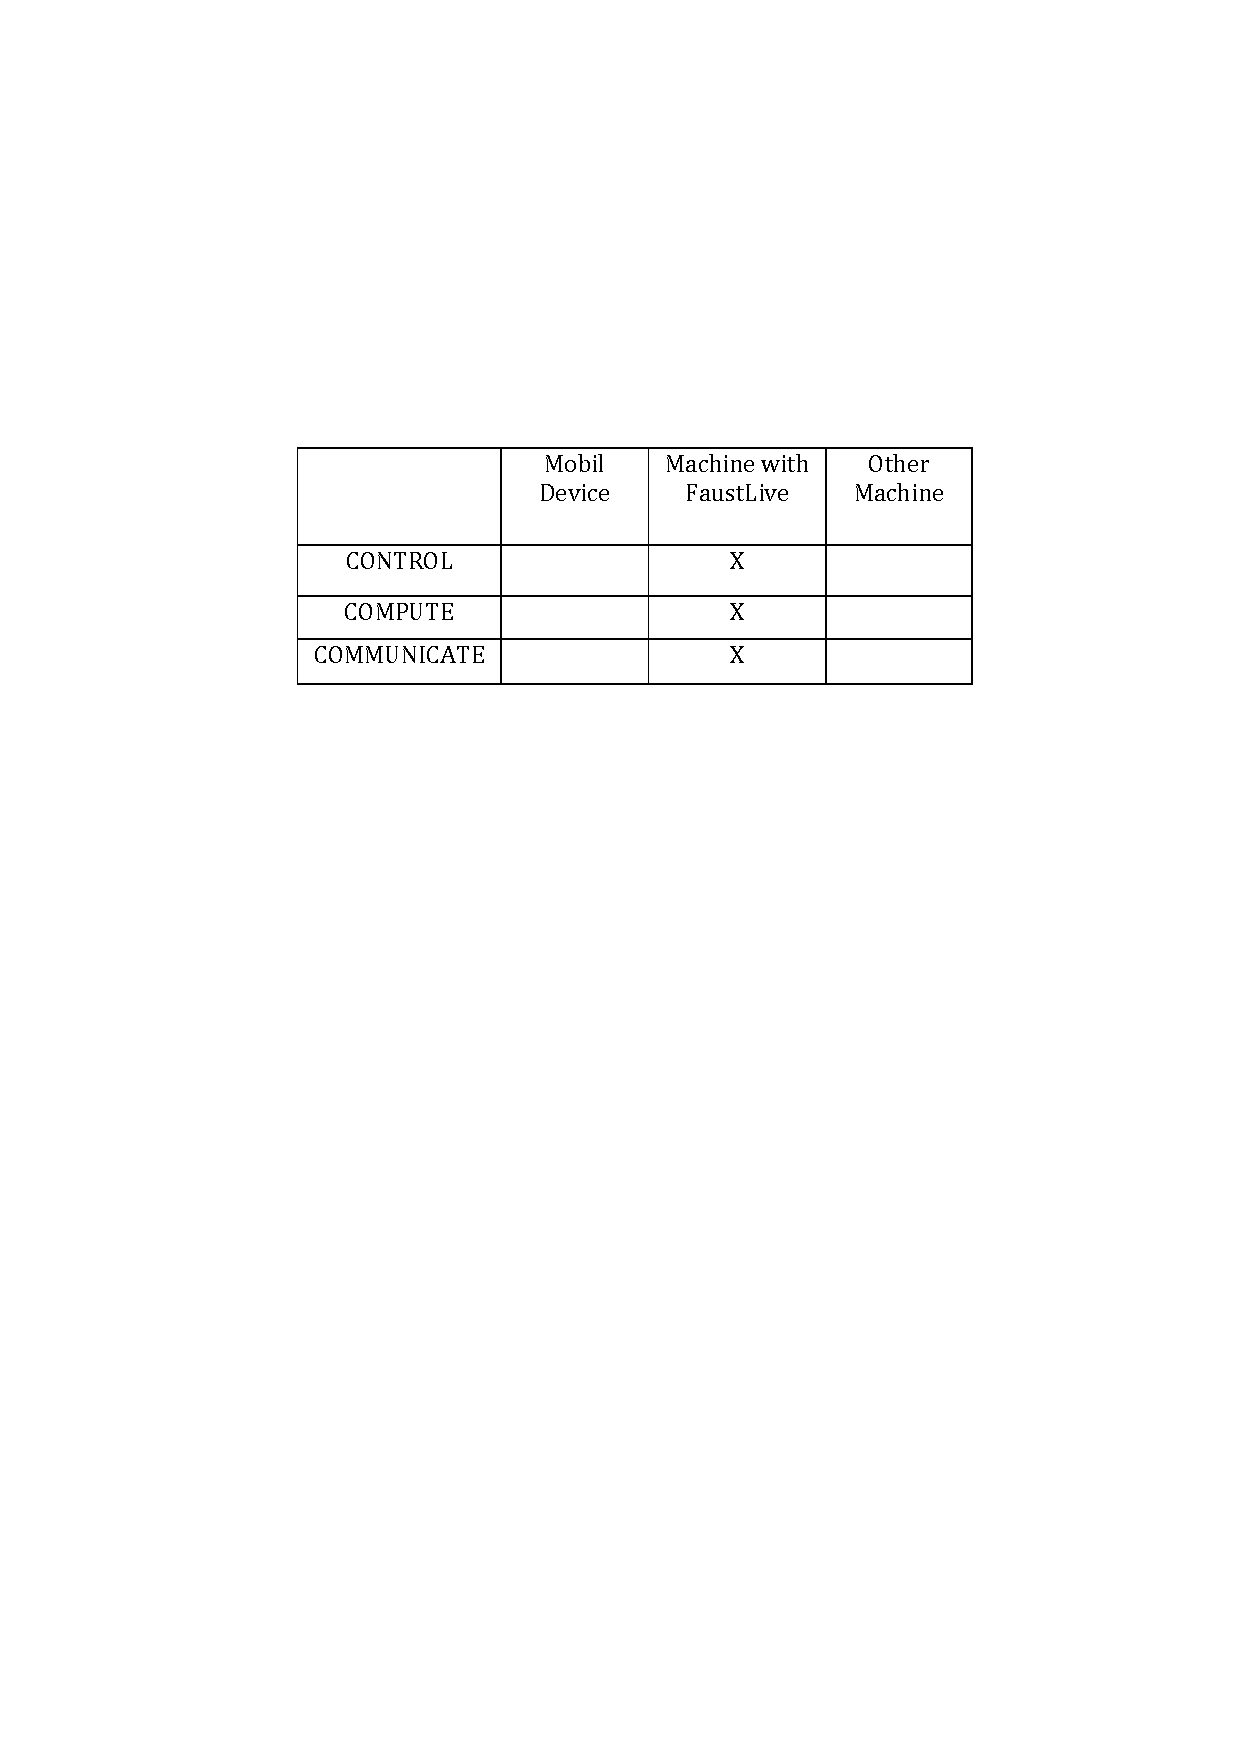
\includegraphics[width=0.7\columnwidth]{images/1CCC}
\caption{Control-Compute-Communicate Division for the main uses of FaustLive}
\label{fig:1CCC}
\end{center}
\end{figure}

\begin{figure}[!h]
\begin{center}
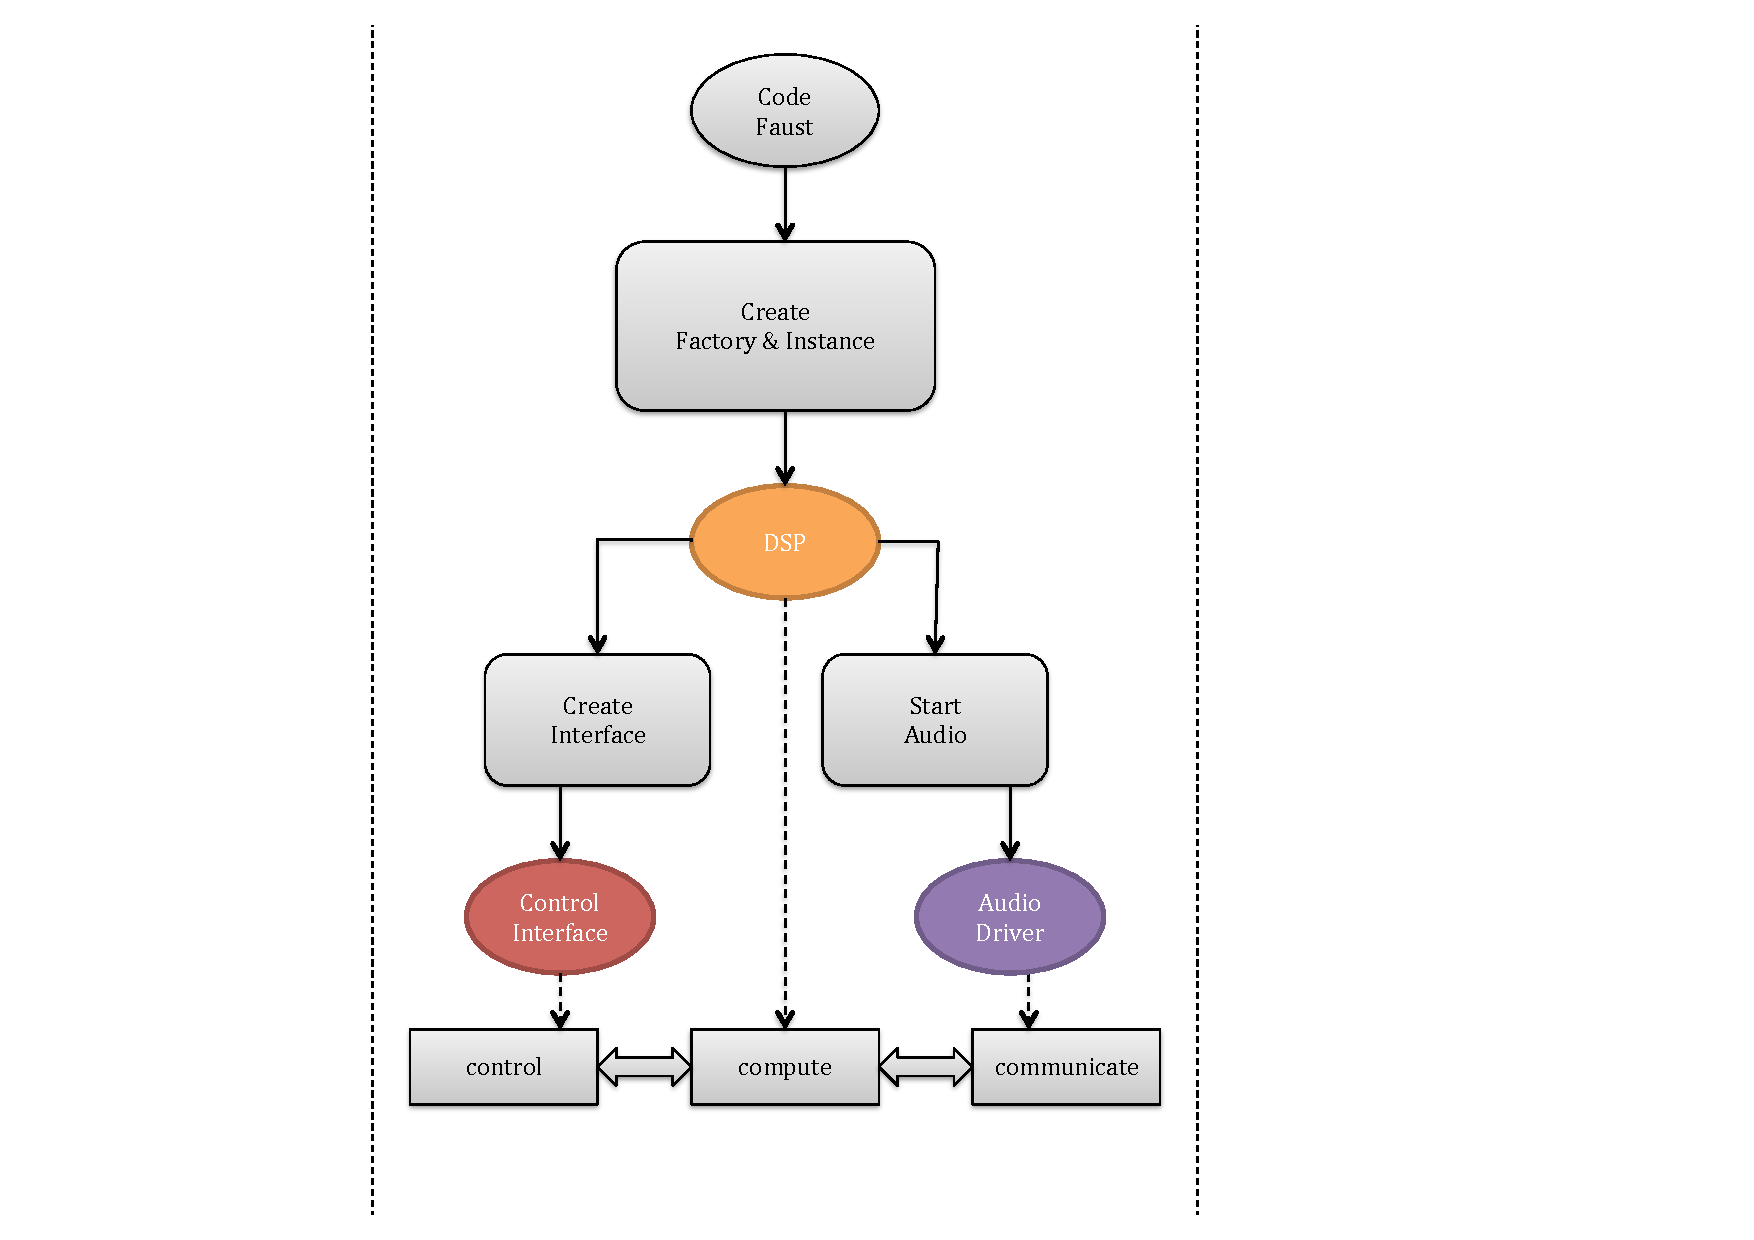
\includegraphics[width=\columnwidth]{images/CCC1}
\caption{Creation of the Interface/DSP/Driver for the main uses of FaustLive}
\label{fig:CCC1}
\end{center}
\end{figure}

%%%%%%%%%%%%%%REMOTE CONTROL%%%%%%%%%%%%%%%%%
\newpage
\subsection{ Using the remote control (OSC, HTTP or other?)} \label{remotecontrol}
In FaustLive, you can create an OSC or an HTTP interface for each window in the window toolbar.
A shortcut to creating an HTTP interface is requesting the QrCode corresponding to the window. This qrcode is a shortcut to the remote control interface. \\

An idea implemented for HTTP remote interfaces but not OSC:
\begin{itemize}
\item The mobile device sends code to create the factory then gets back the interface while the processing and rendering are done in FaustLive.
\end{itemize}

\begin{figure}[!h]
\begin{center}
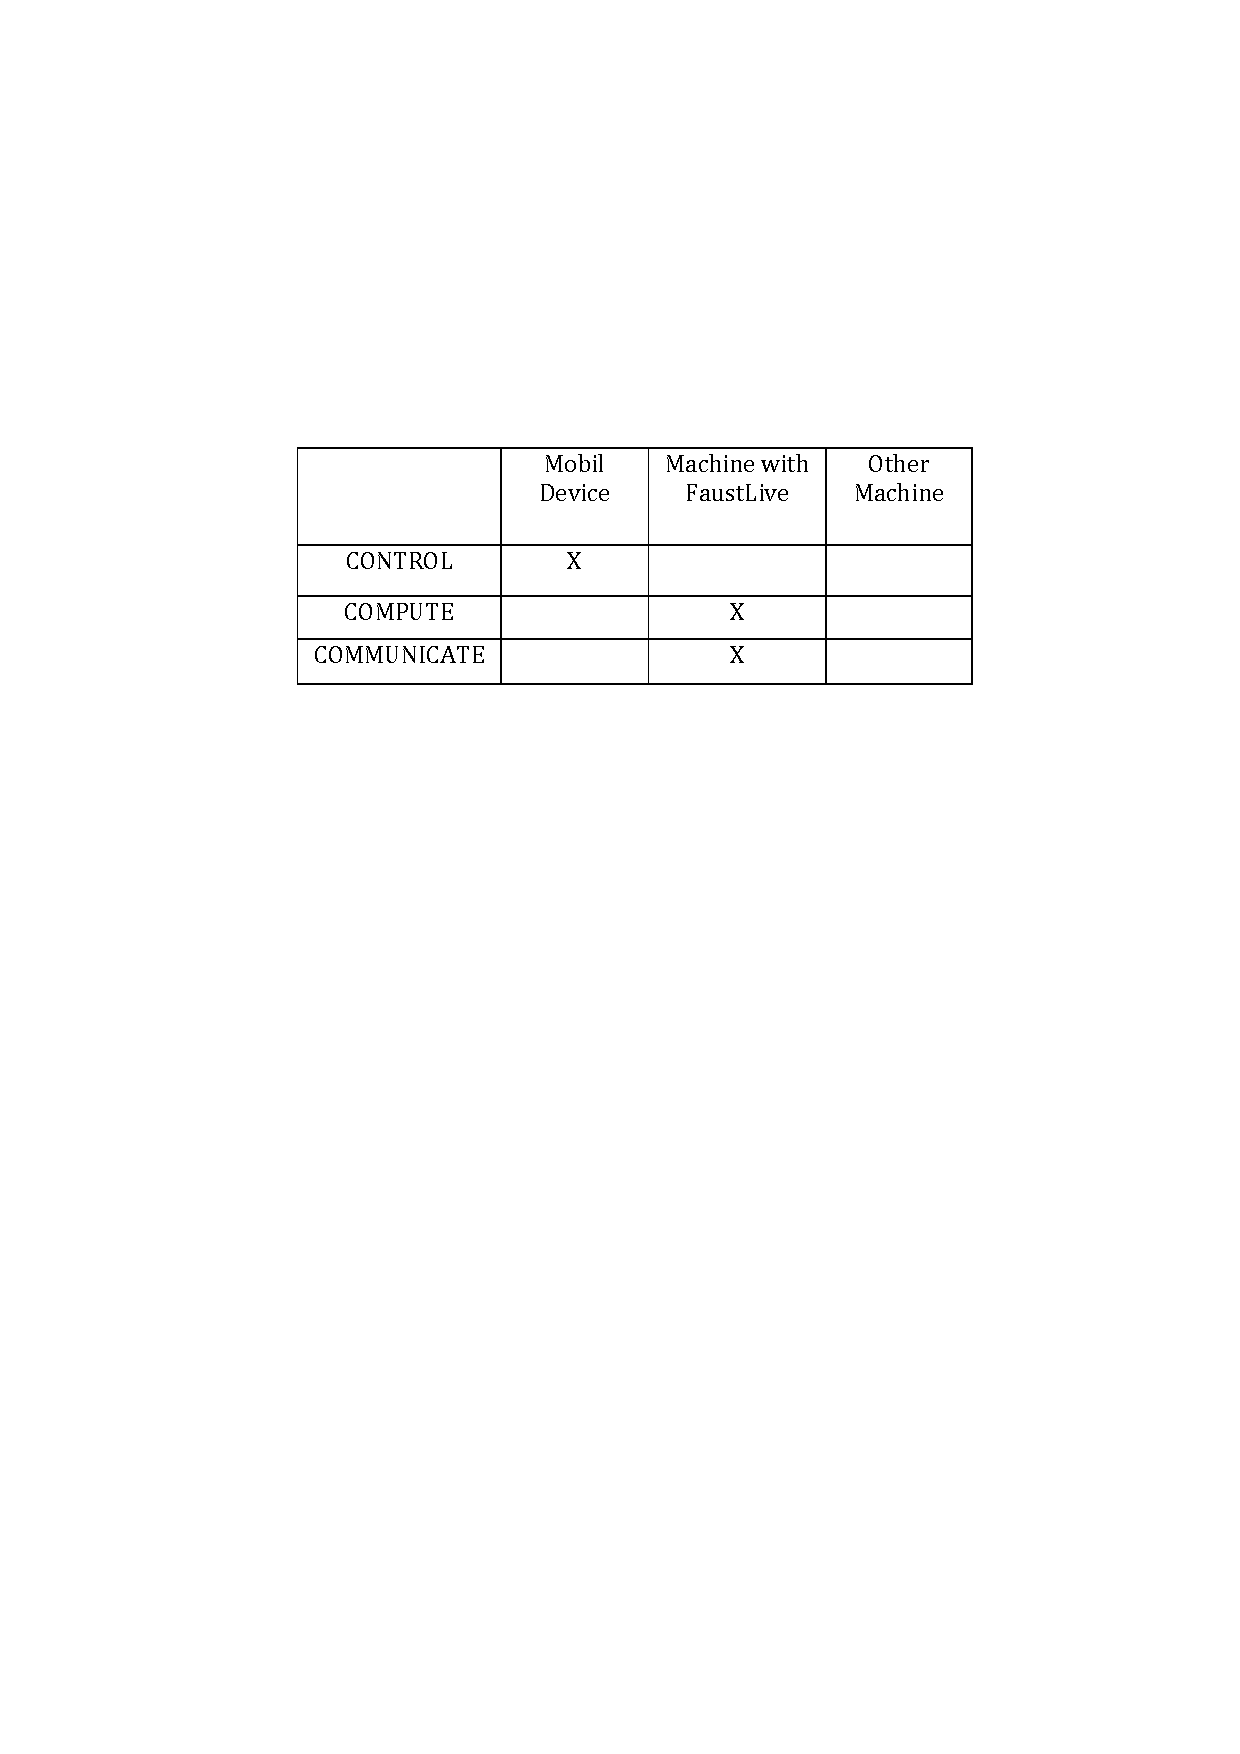
\includegraphics[width=0.7\columnwidth]{images/2CCC}
\caption{Control-Compute-Communicate Division with remote interface}
\label{fig:2CCC}
\end{center}
\end{figure}
\begin{figure}[!h]
\begin{center}
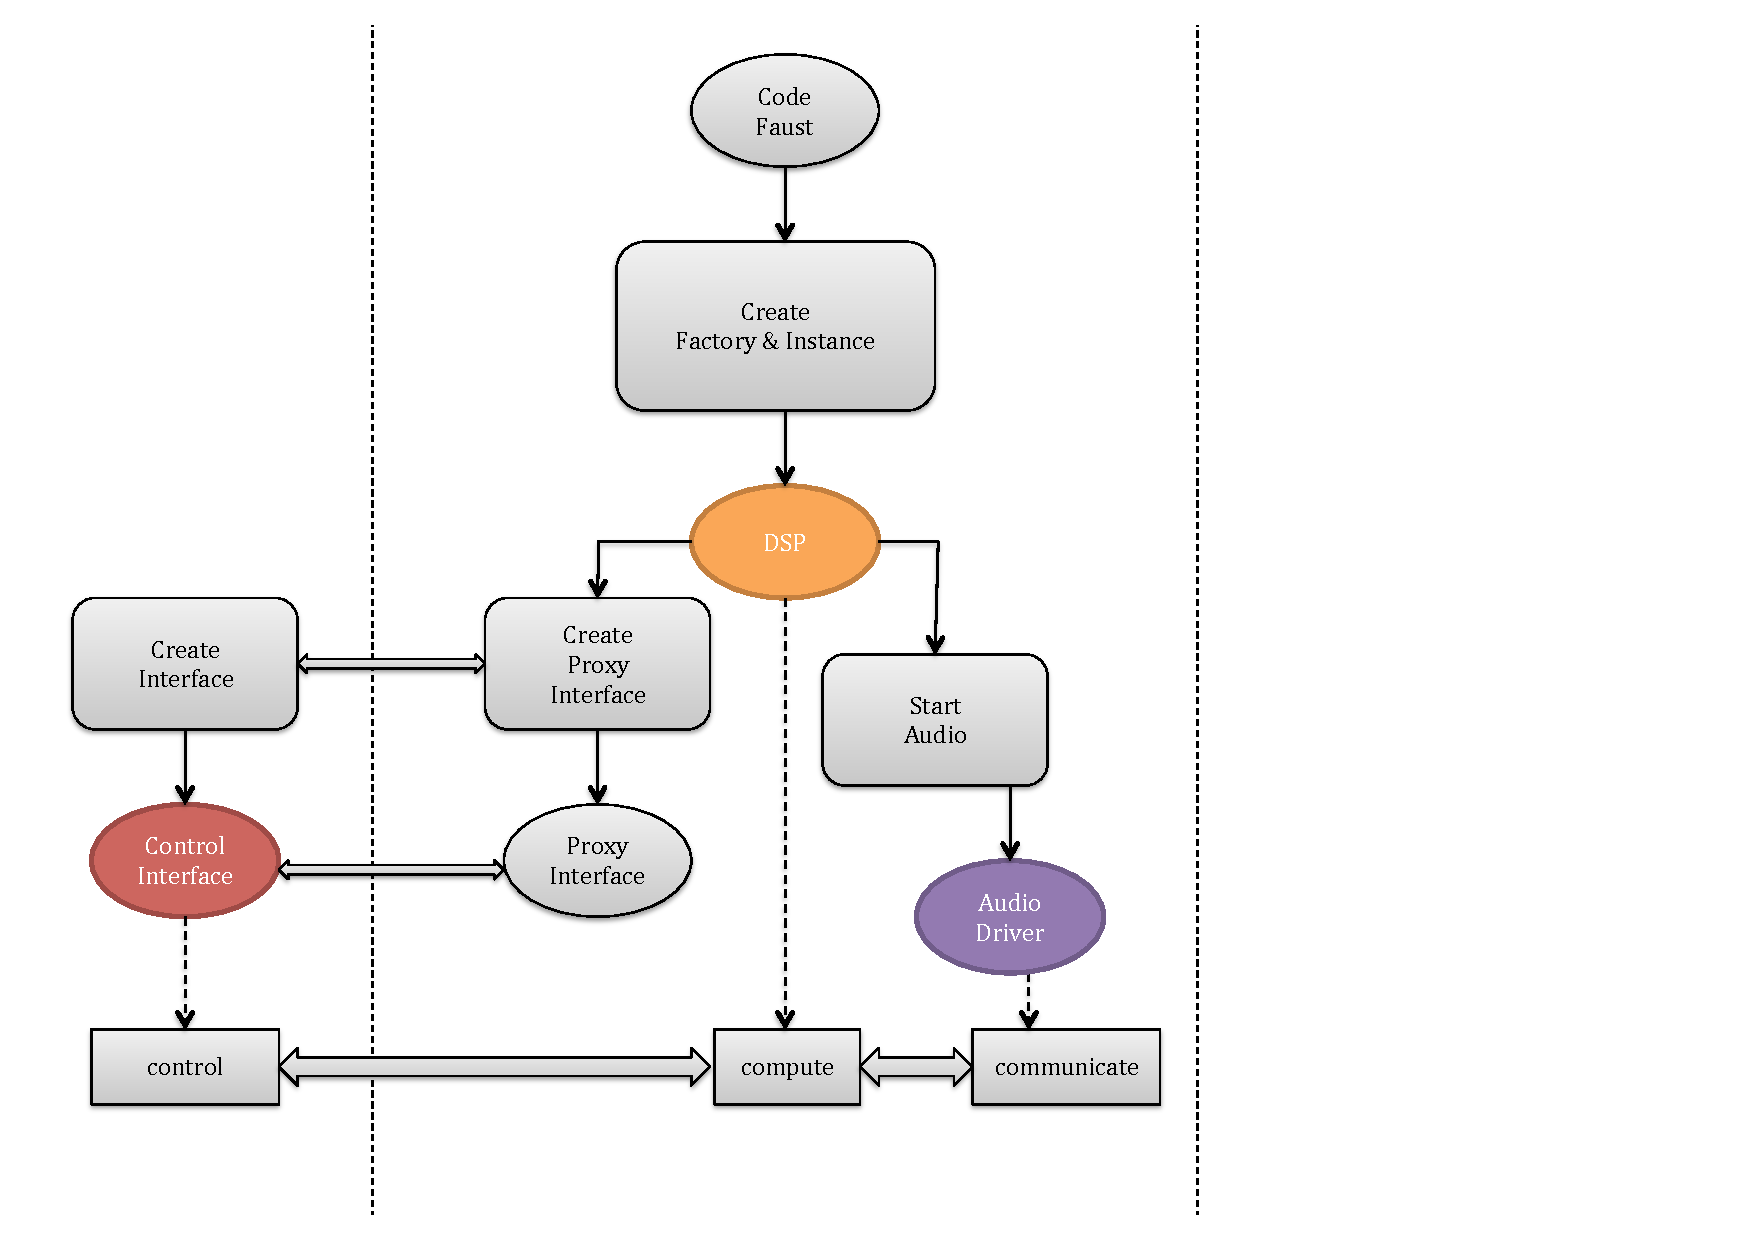
\includegraphics[width=\columnwidth]{images/CCC2}
\caption{Creation of the Interface/DSP/Driver for a remote control use case}
\label{fig:CCC2}
\end{center}
\end{figure}


%%%%%%%%%%%%%%REMOTE RENDER%%%%%%%%%%%%%%%%%
\newpage
\subsection {Using NetJack for remote audio rendering} \label{remoterendering}

In FaustLive, switch to NetJack as audio driver in the general preferences. 
\begin{figure}[!h]
\begin{center}
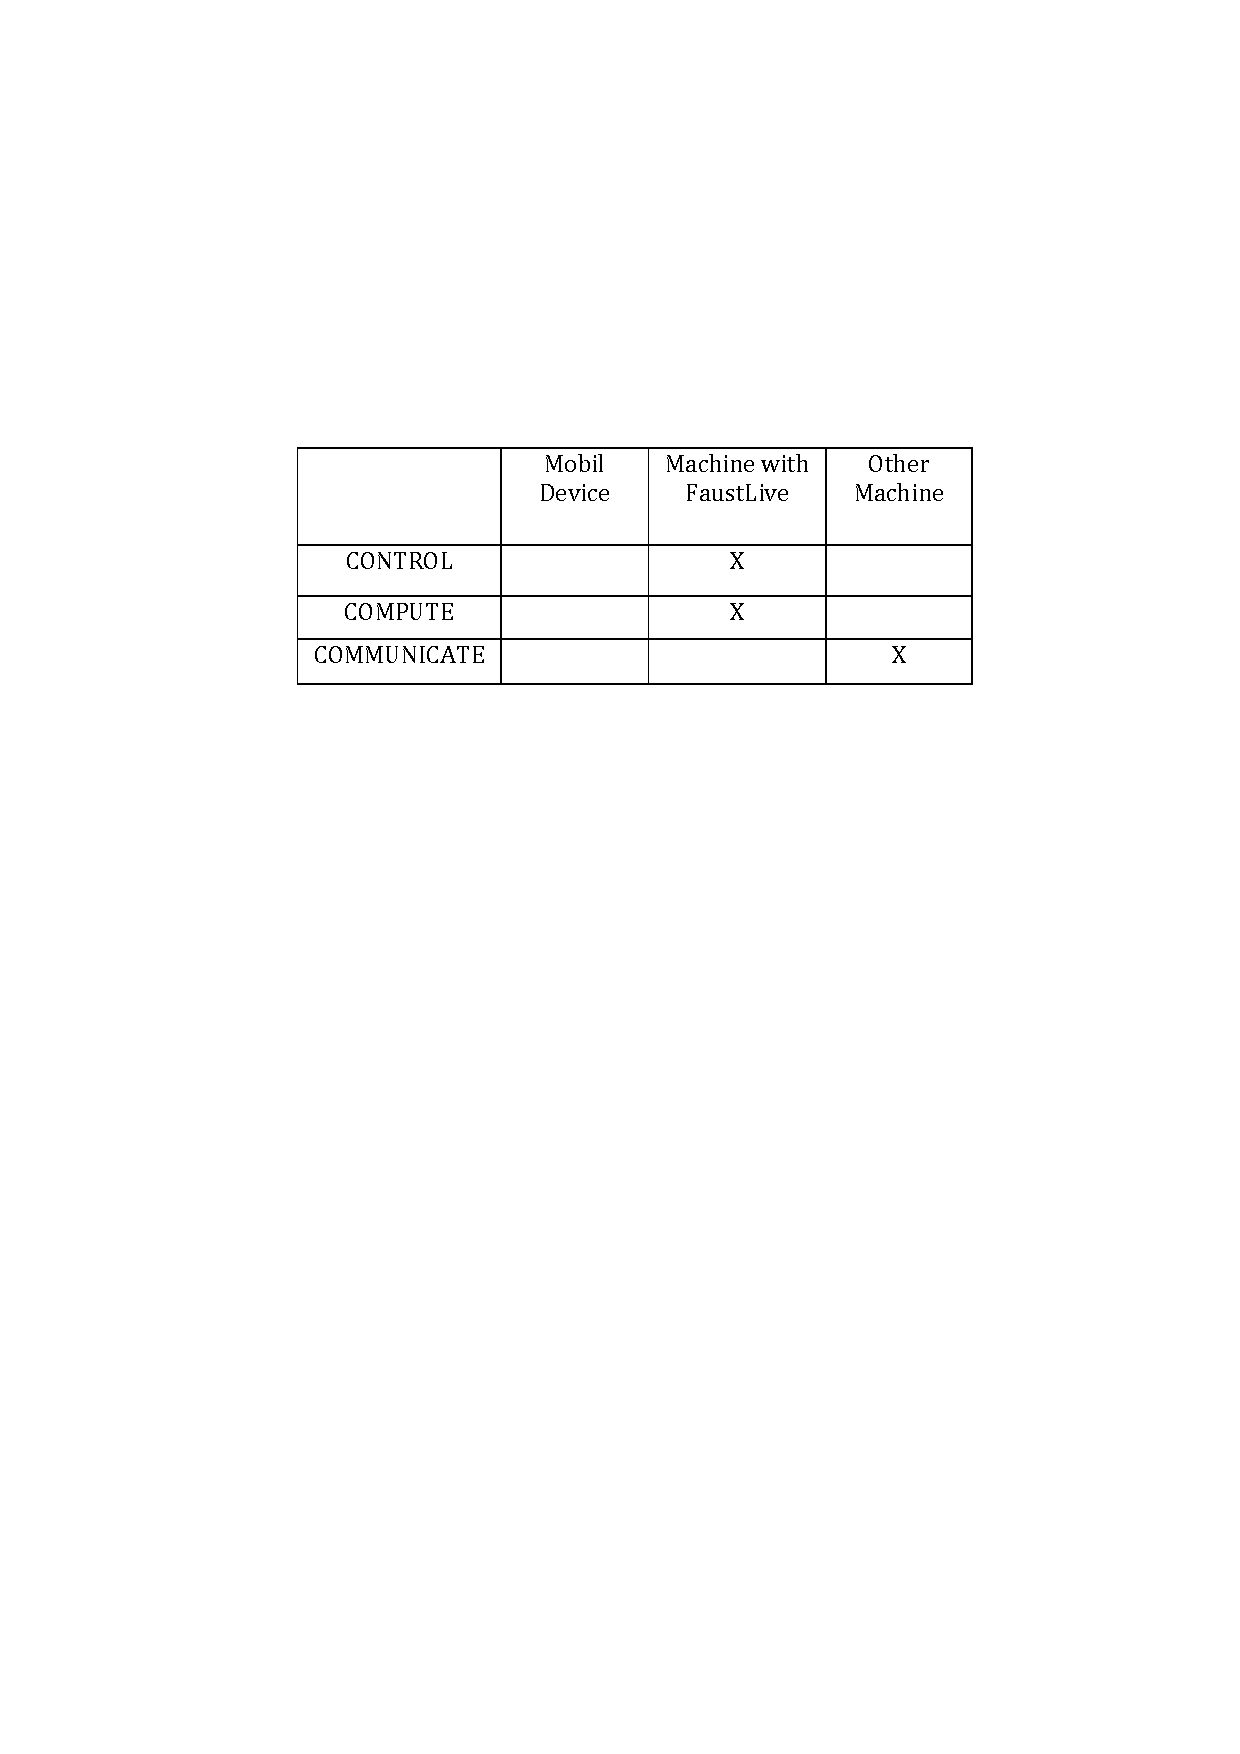
\includegraphics[width=0.7\columnwidth]{images/3CCC}
\caption{Control-Compute-Communicate Division with remote audio rendering}
\label{fig:3CCC}
\end{center}
\end{figure}
\begin{figure}[!h]
\begin{center}
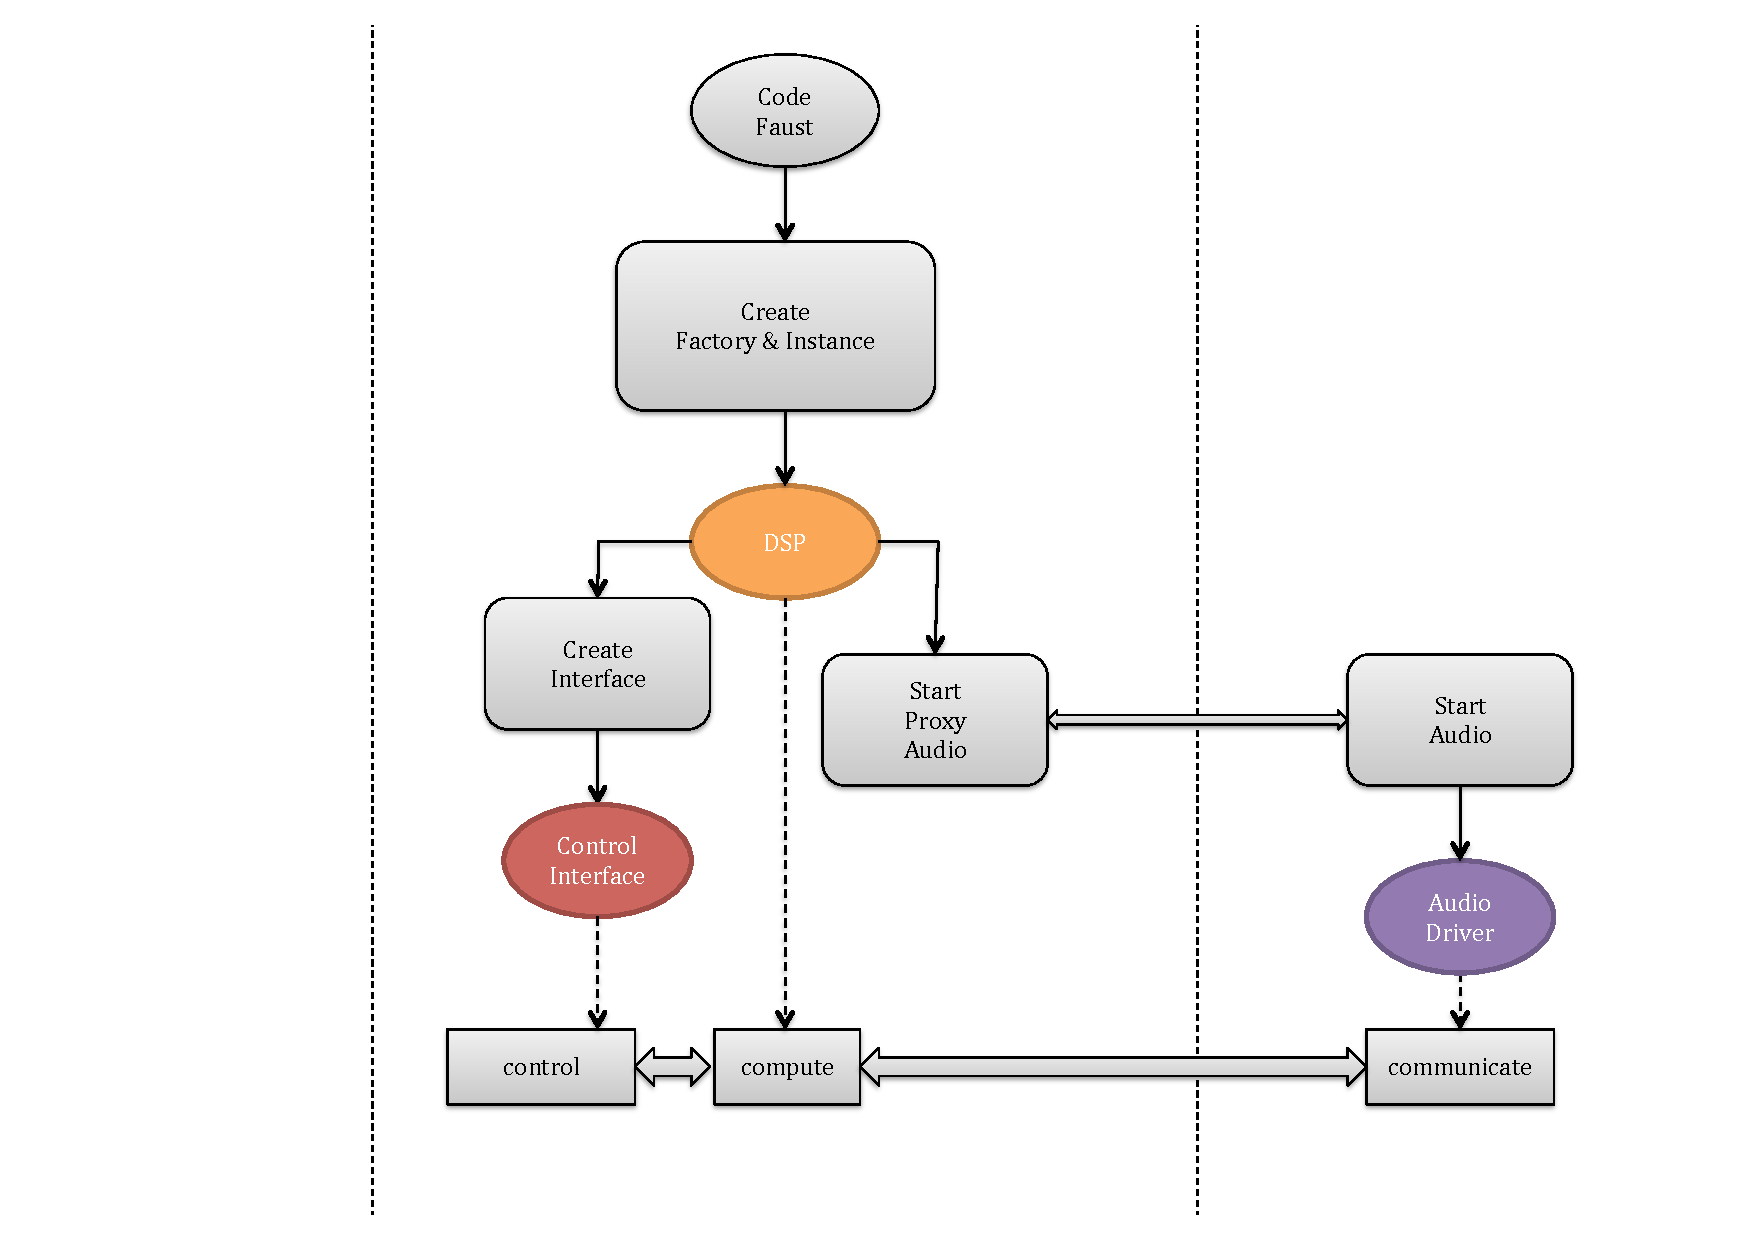
\includegraphics[width=\columnwidth]{images/CCC3}
\caption{Creation of the Interface/DSP/Driver for a remote rendering use case}
\label{fig:CCC2}
\end{center}
\end{figure}
%%%%%%%%%%%%%%REMOTE CONTROL & RENDER%%%%%%%%%%%%%%%%%
\newpage
\subsection{ Remote control and remote rendering}

Combining use case {\ref{remotecontrol}} and use case {\ref{remoterendering}}.

\begin{figure}[!h]
\begin{center}
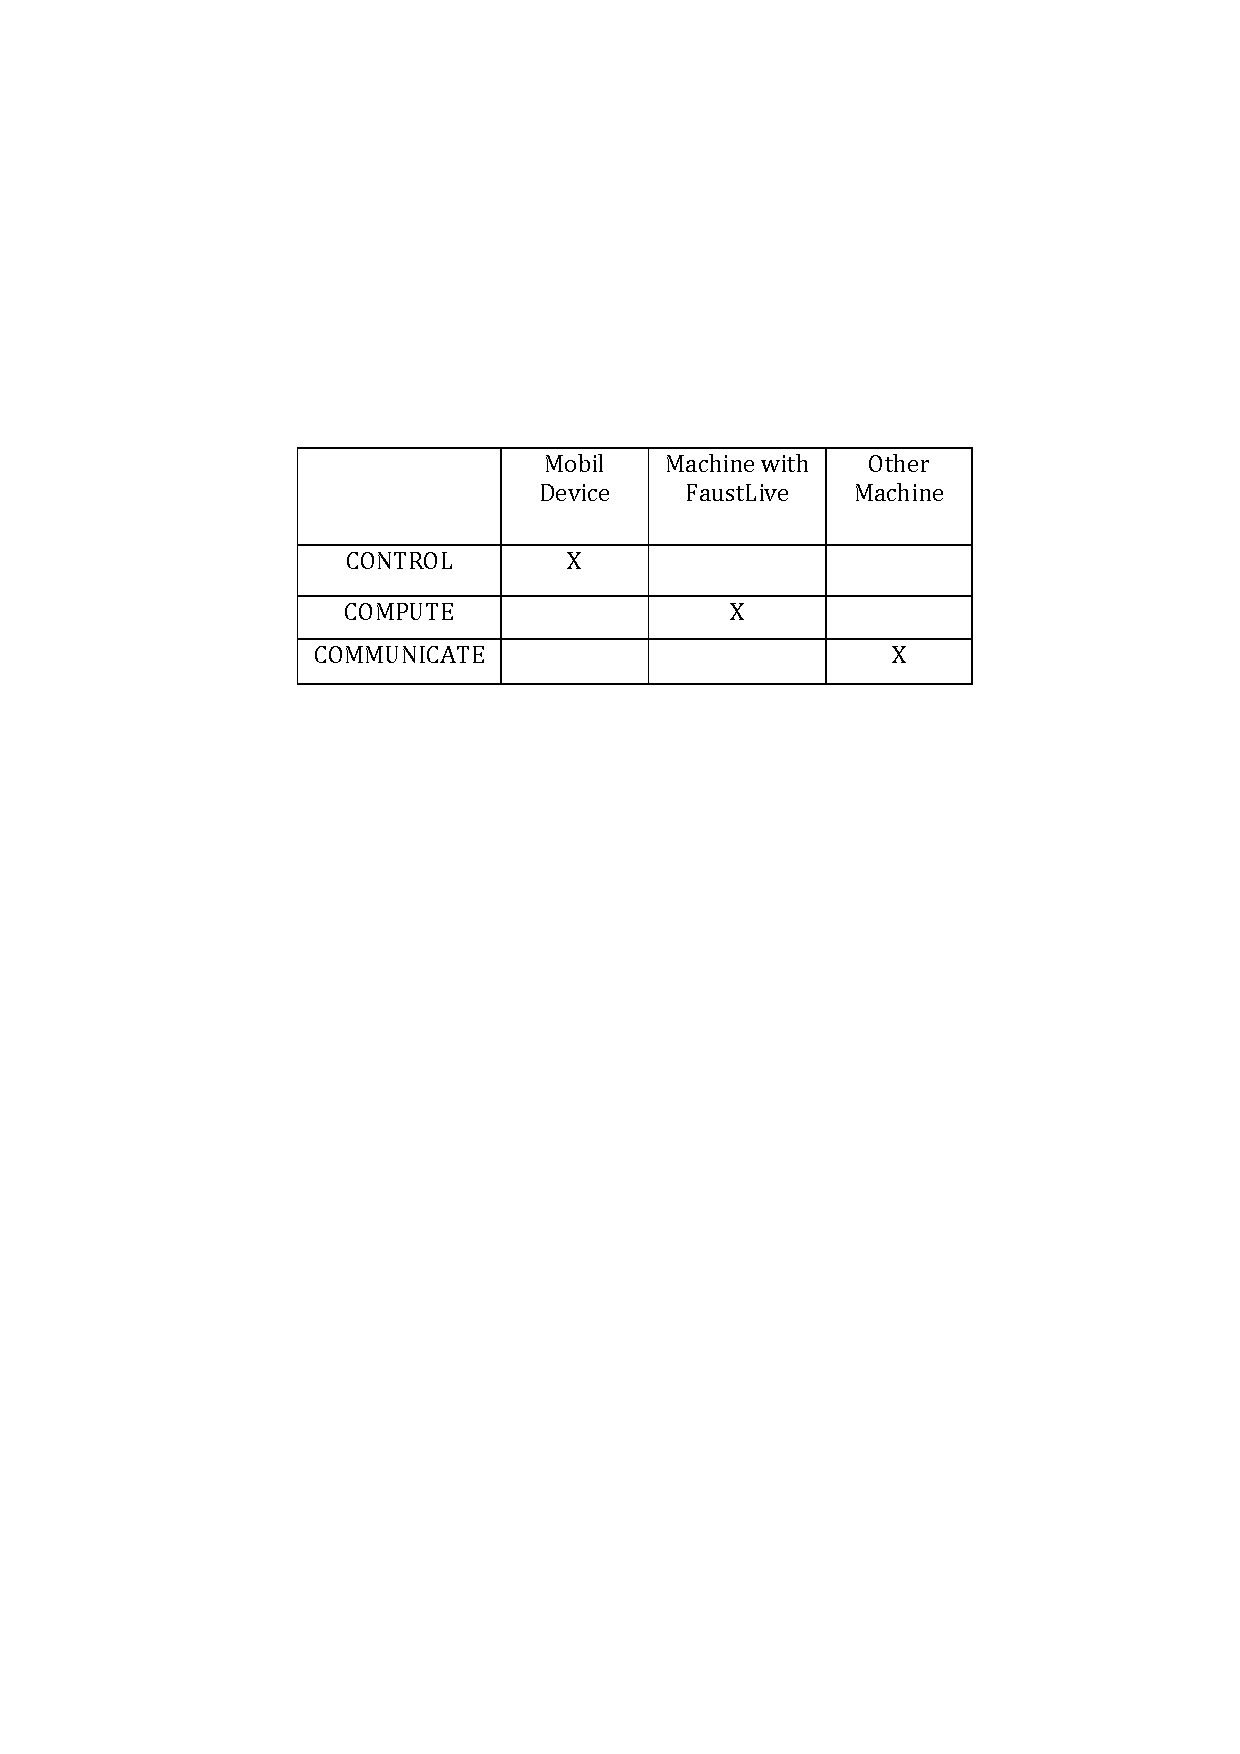
\includegraphics[width=0.7\columnwidth]{images/8CCC}
\caption{Control-Compute-Communicate Division with remote control and remote audio rendering}
\label{fig:8CCC}
\end{center}
\end{figure}
\begin{figure}[!h]
\begin{center}
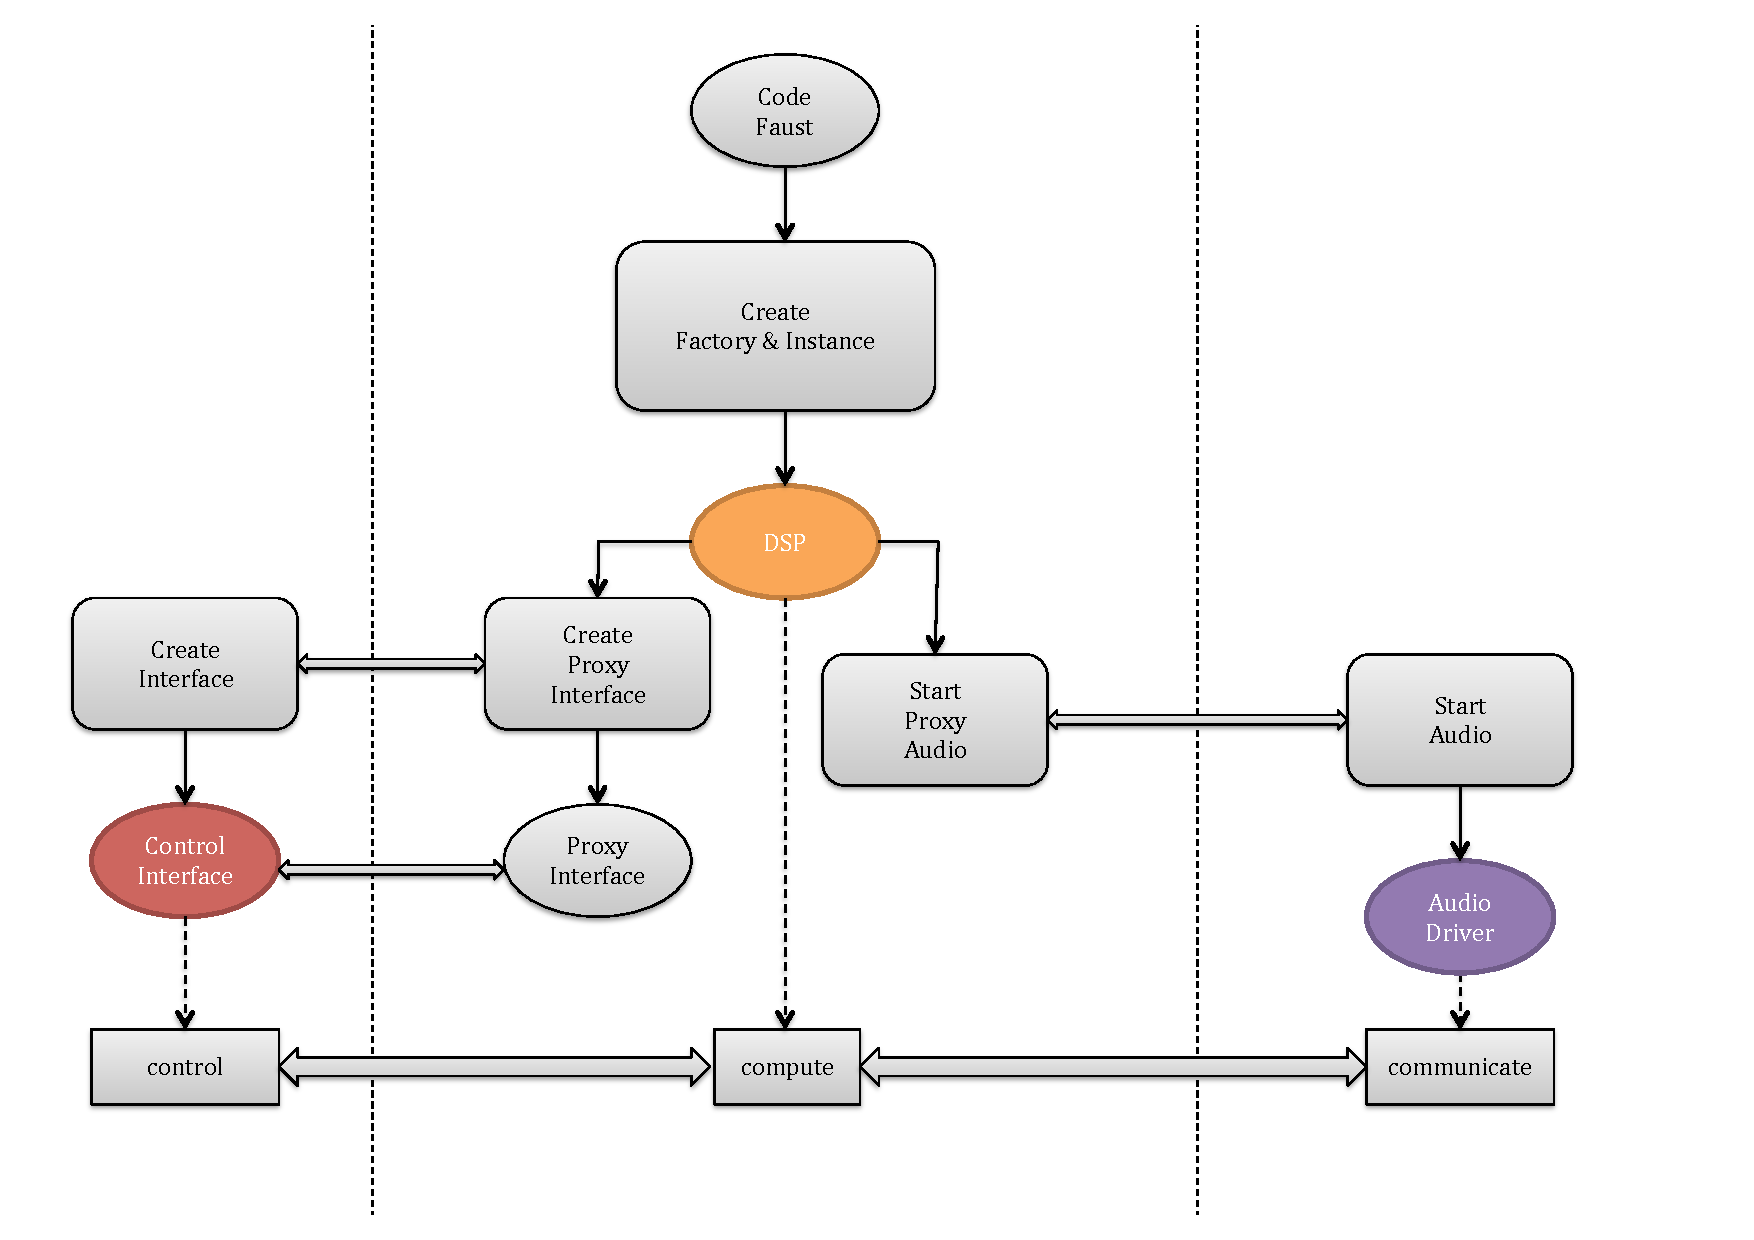
\includegraphics[width=\columnwidth]{images/CCC8}
\caption{Creation of the Interface/DSP/Driver for a remote control and rendering use case}
\label{fig:CCC8}
\end{center}
\end{figure}

%%%%%%%%%%%%%%REMOTE PROCESSING%%%%%%%%%%%%%%%%%
\newpage
\subsection {Remote processing} \label{remoteprocessing}

1 use case is implemented in FaustLive:
\begin{itemize}
\item FaustLive sends code to create a remote factory then has the control and communicate parts 
\end{itemize}
You can access this use case through the scrolling menu containing the available servers below the window. \\

The 2nd use case is conceivable but not implemented:
\begin{itemize}
\item FaustLive discovers remote factories and requests a remote instance then has the control and communicate aspects over it
\end{itemize}

\begin{figure}[!h]
\begin{center}
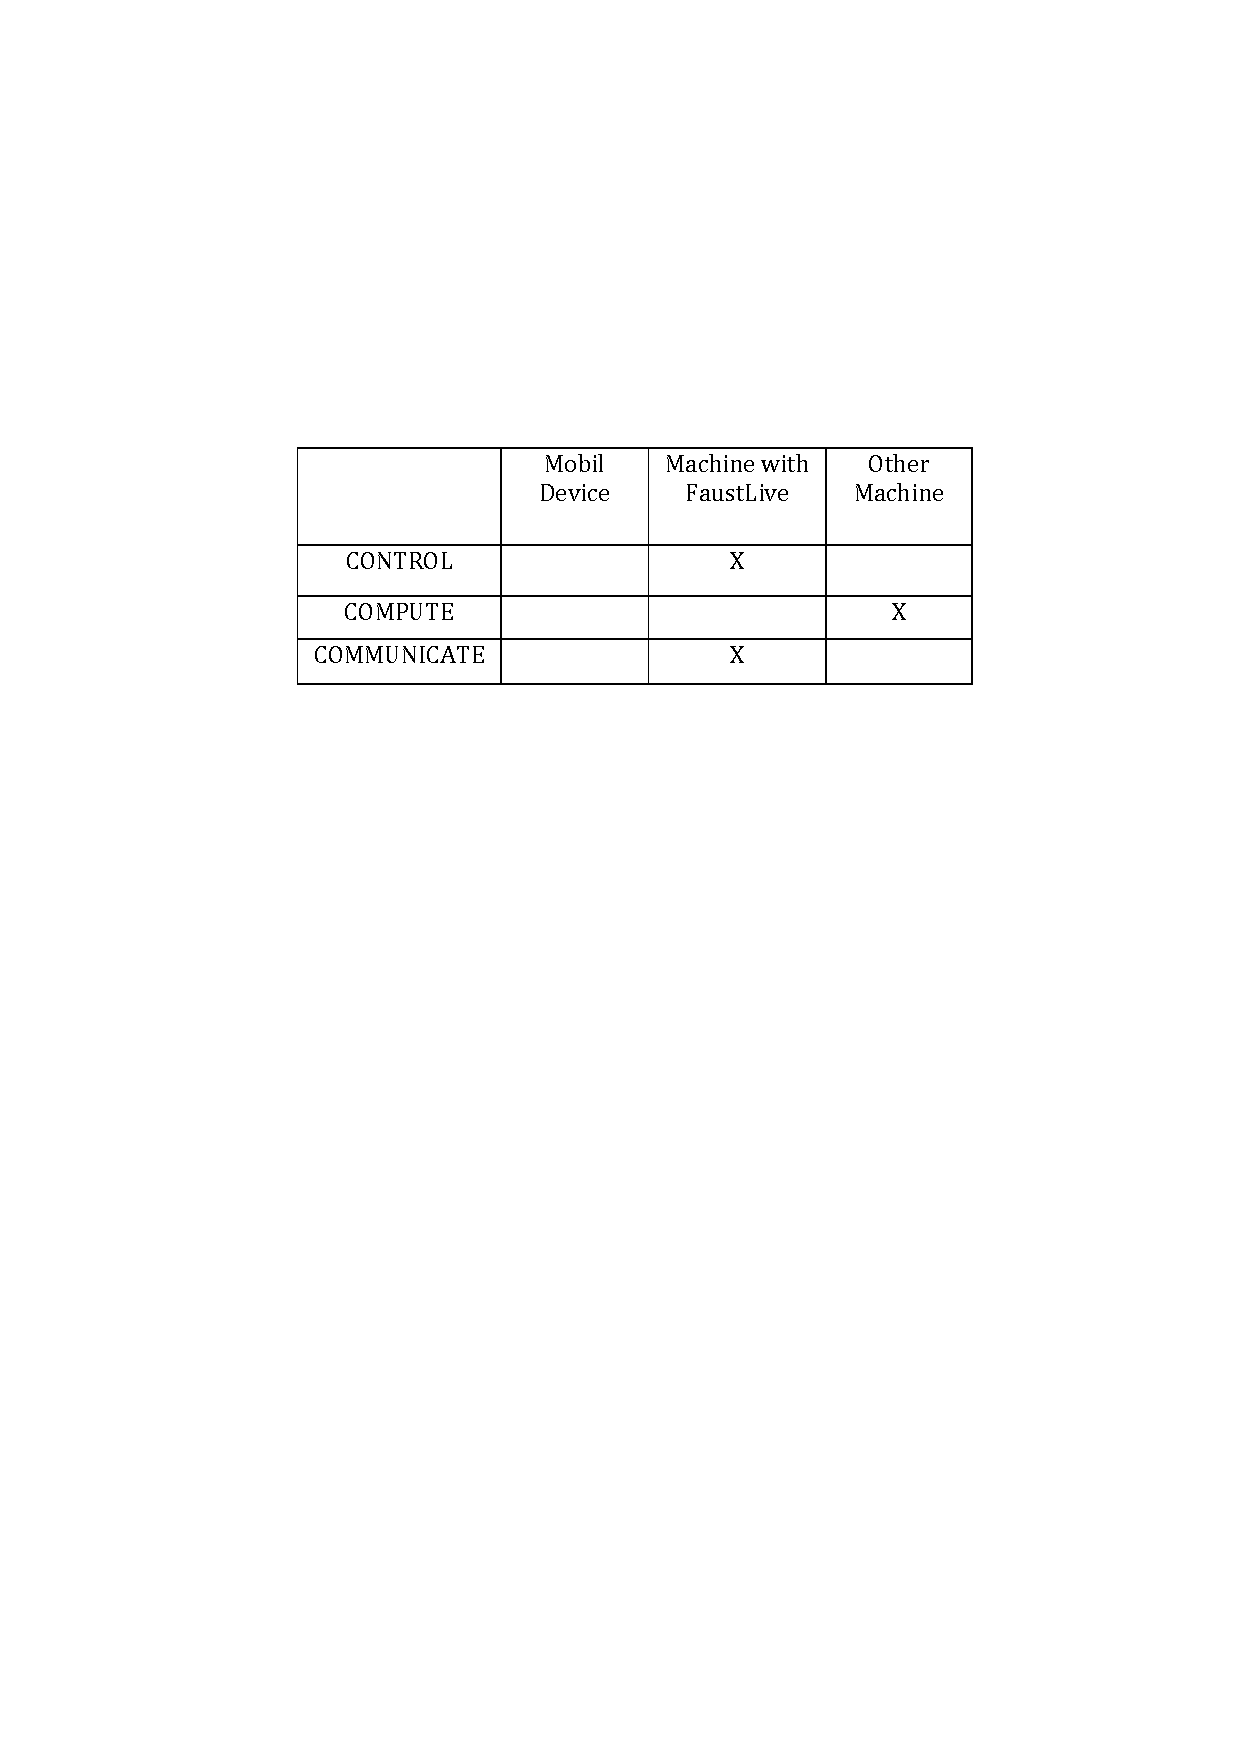
\includegraphics[width=0.7\columnwidth]{images/4CCC}
\caption{Control-Compute-Communicate Division with remote processing}
\label{fig:4CCC}
\end{center}
\end{figure}
\begin{figure}[!h]
\begin{center}

\begin{minipage}[c]{.45\linewidth}
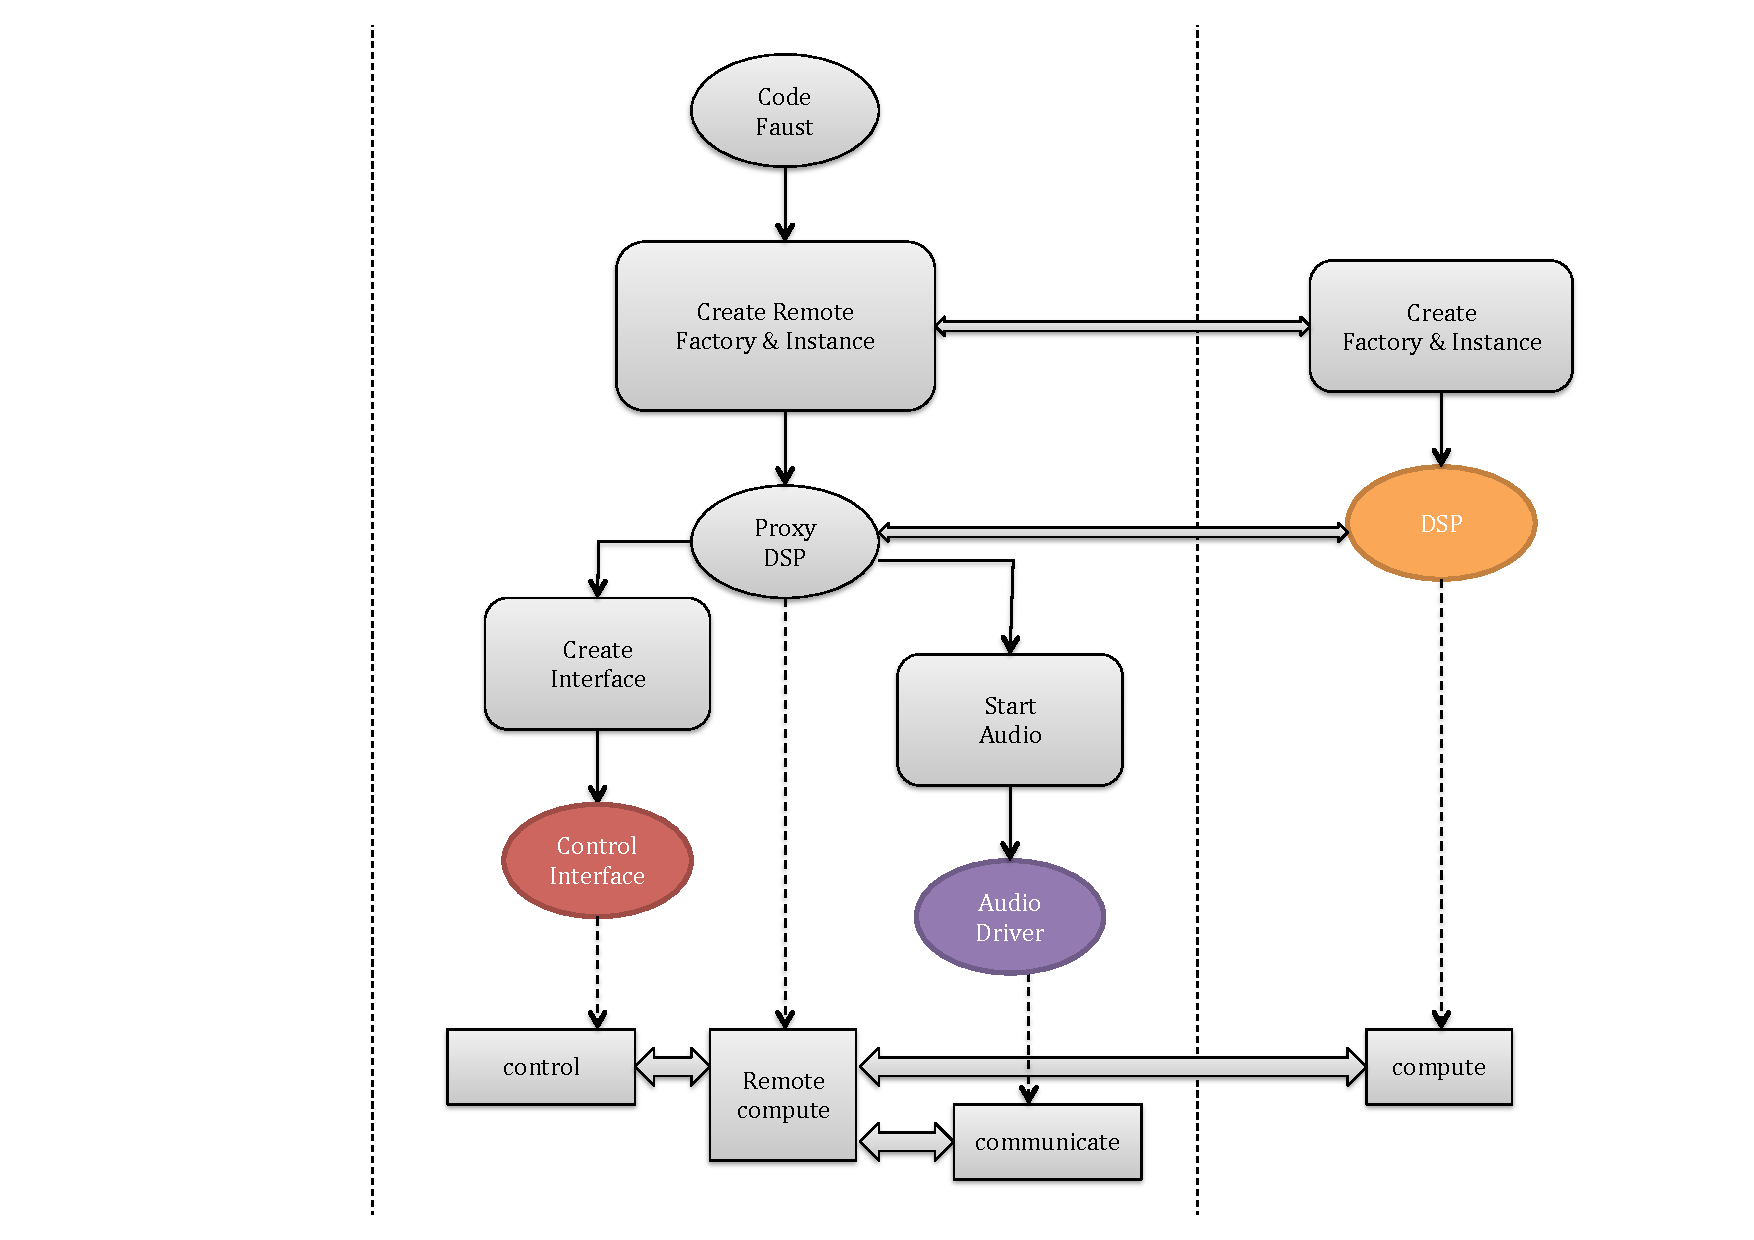
\includegraphics[width=\columnwidth]{images/CCC41}
\end{minipage}
\begin{minipage}[r]{.45\linewidth}
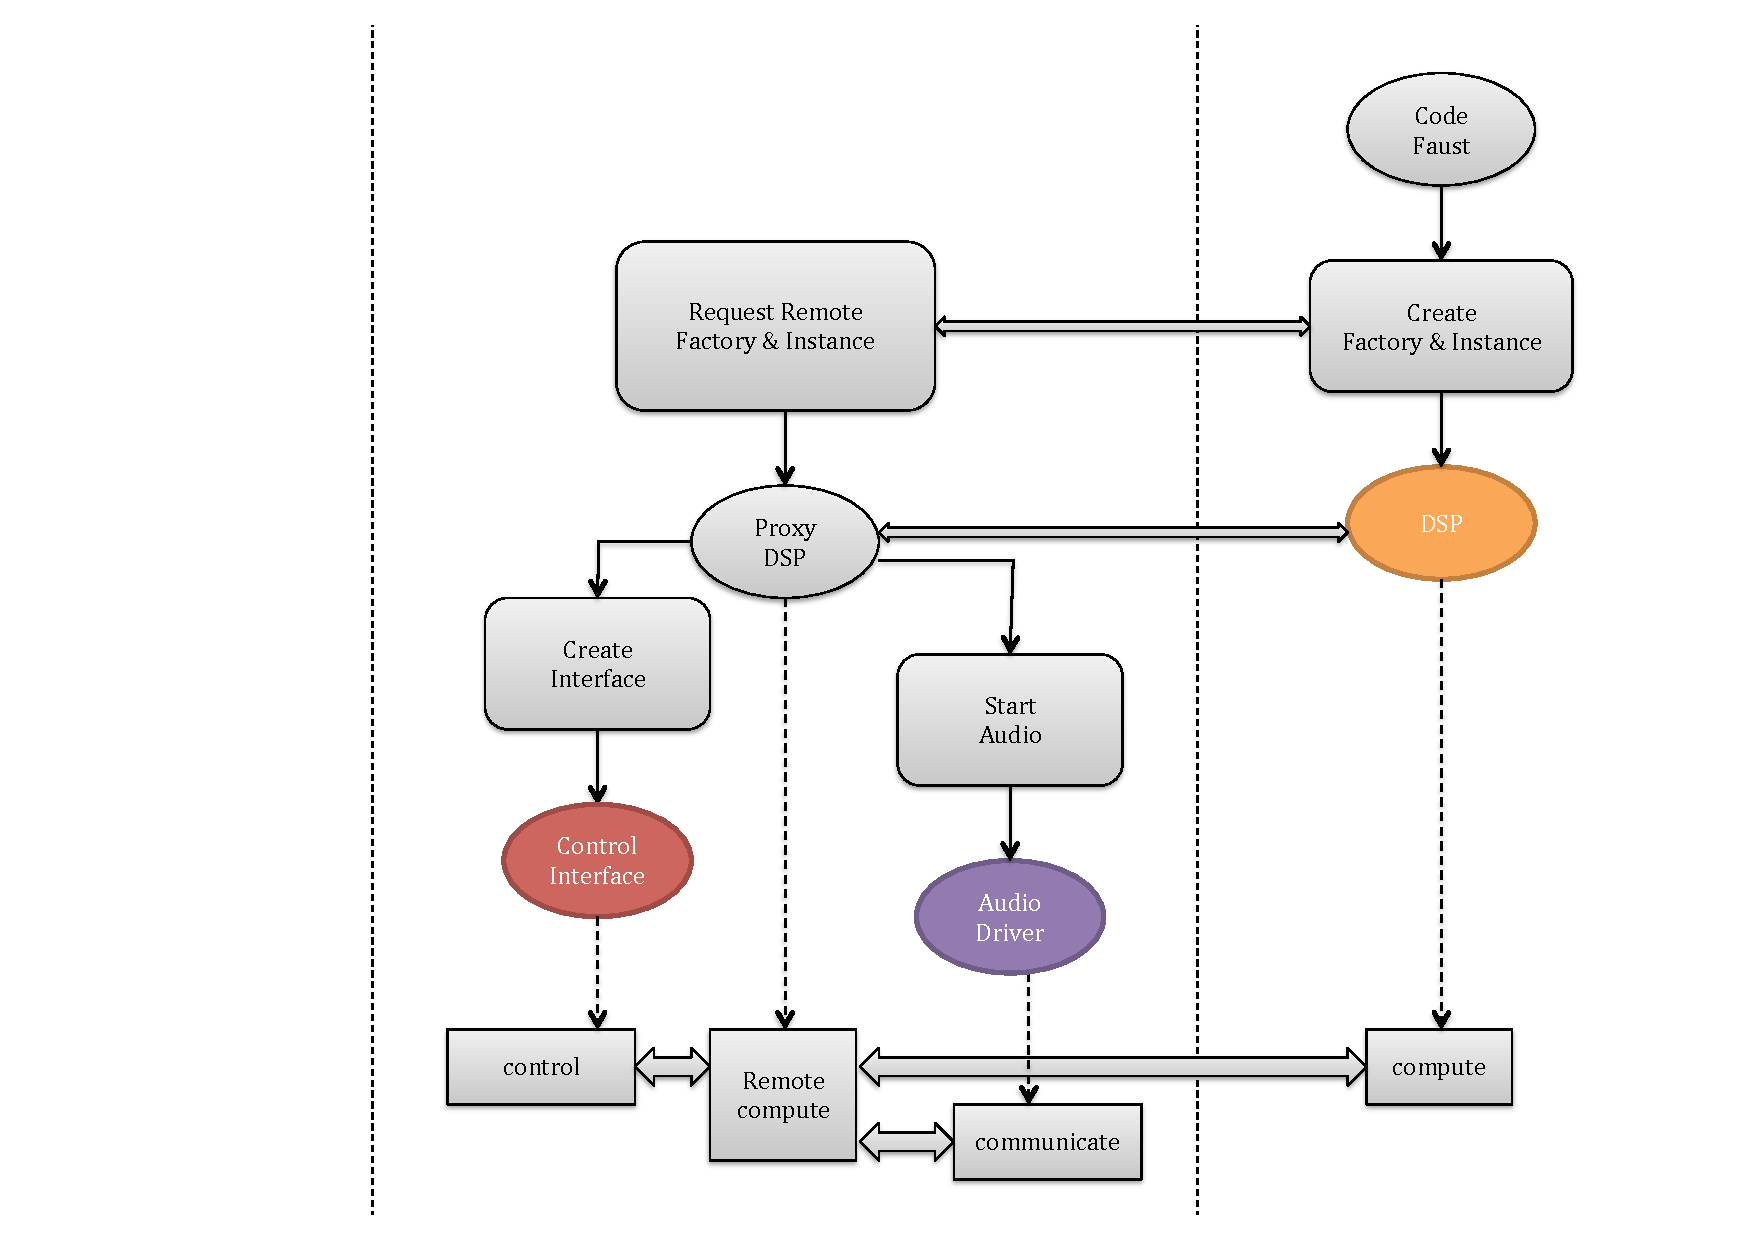
\includegraphics[width=\columnwidth]{images/CCC42}
\end{minipage}
\caption{Creation of the Interface/DSP/Driver for a remote processing use case}
\label{fig:CCC4}
\end{center}
\end{figure}

%%%%%%%%%%%%%%REMOTE PROCESSING AND CONTROL%%%%%%%%%%%%%%%%%
\newpage
\subsection{ Remote processing and remote control}

Combining use case {\ref{remotecontrol}} and use case {\ref{remoteprocessing}}.

\begin{figure}[!h]
\begin{center}
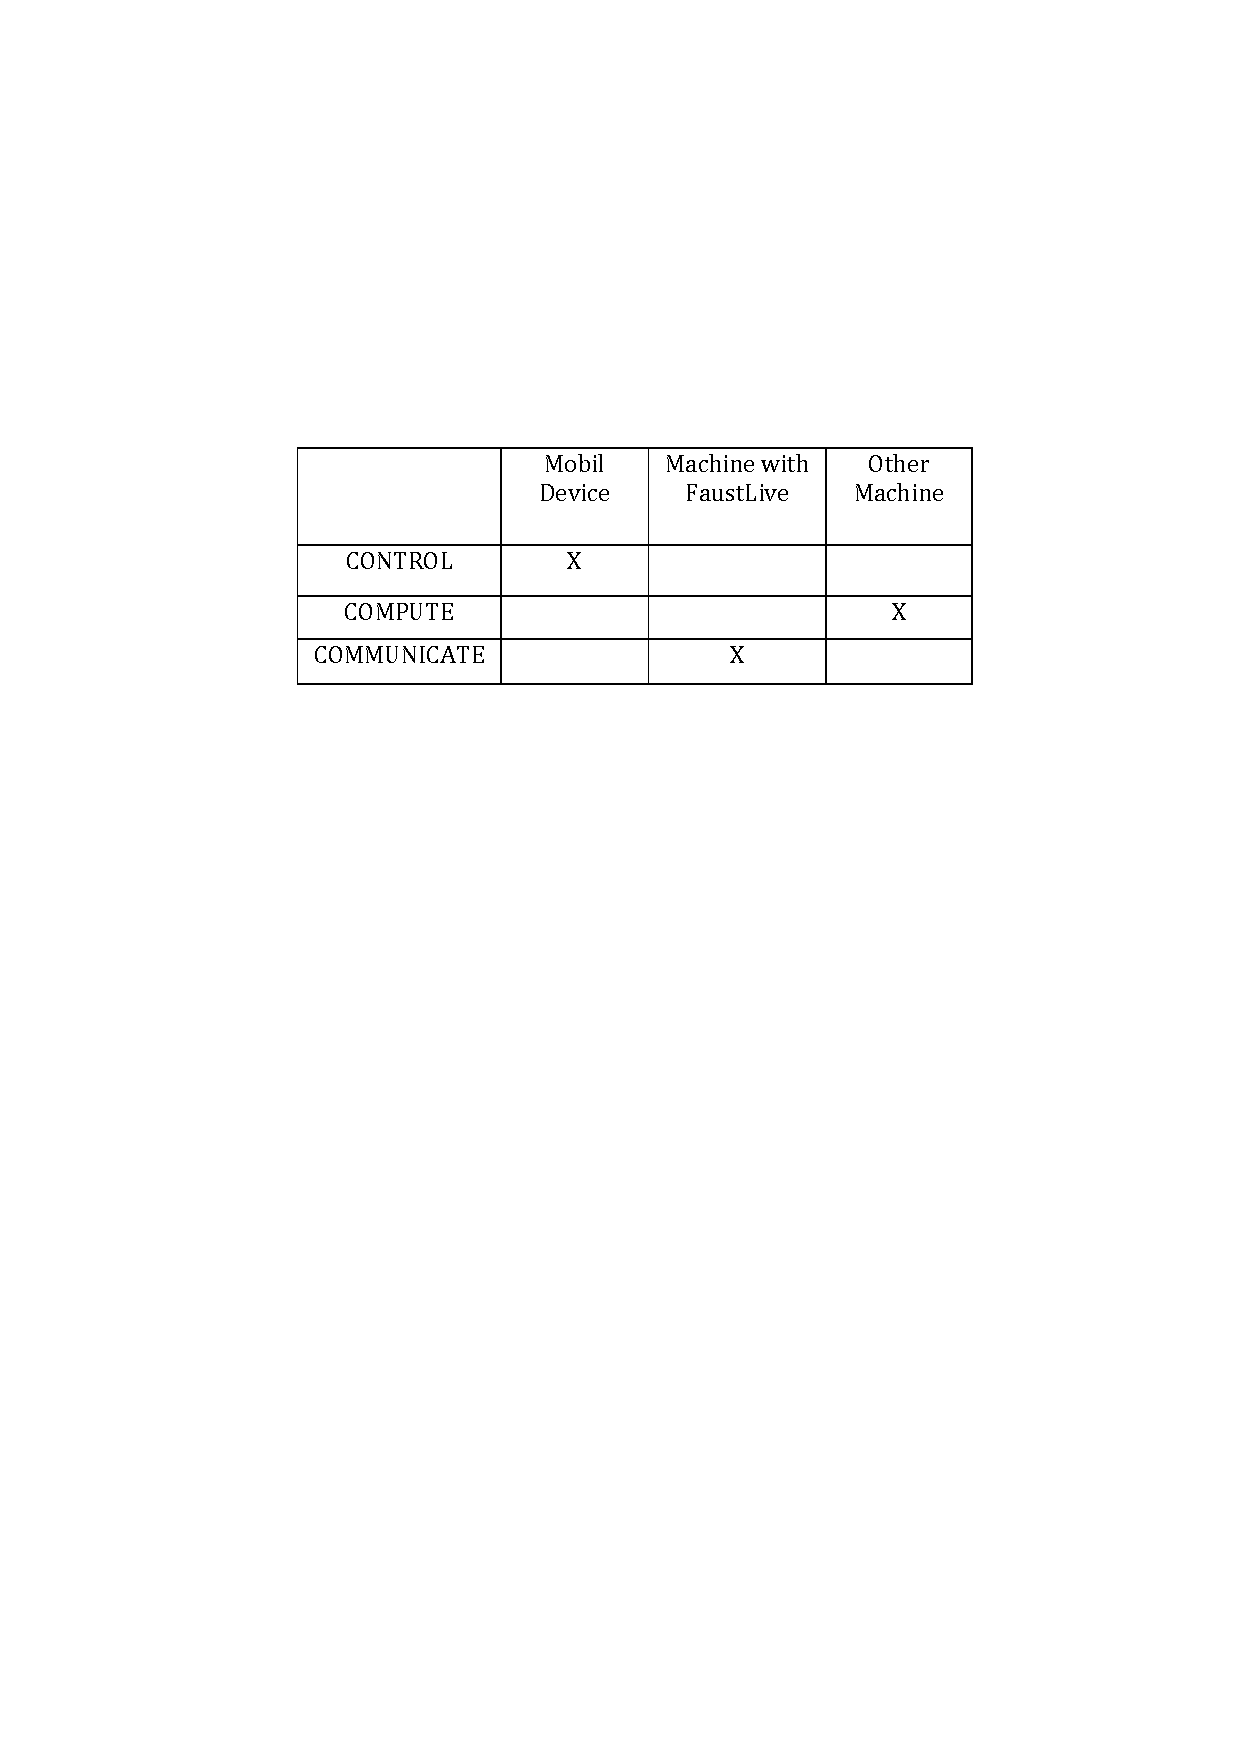
\includegraphics[width=0.7\columnwidth]{images/5CCC}
\caption{Control-Compute-Communicate Division with remote processing and control}
\label{fig:5CCC}
\end{center}
\end{figure}

\begin{figure}[!h]
\begin{center}
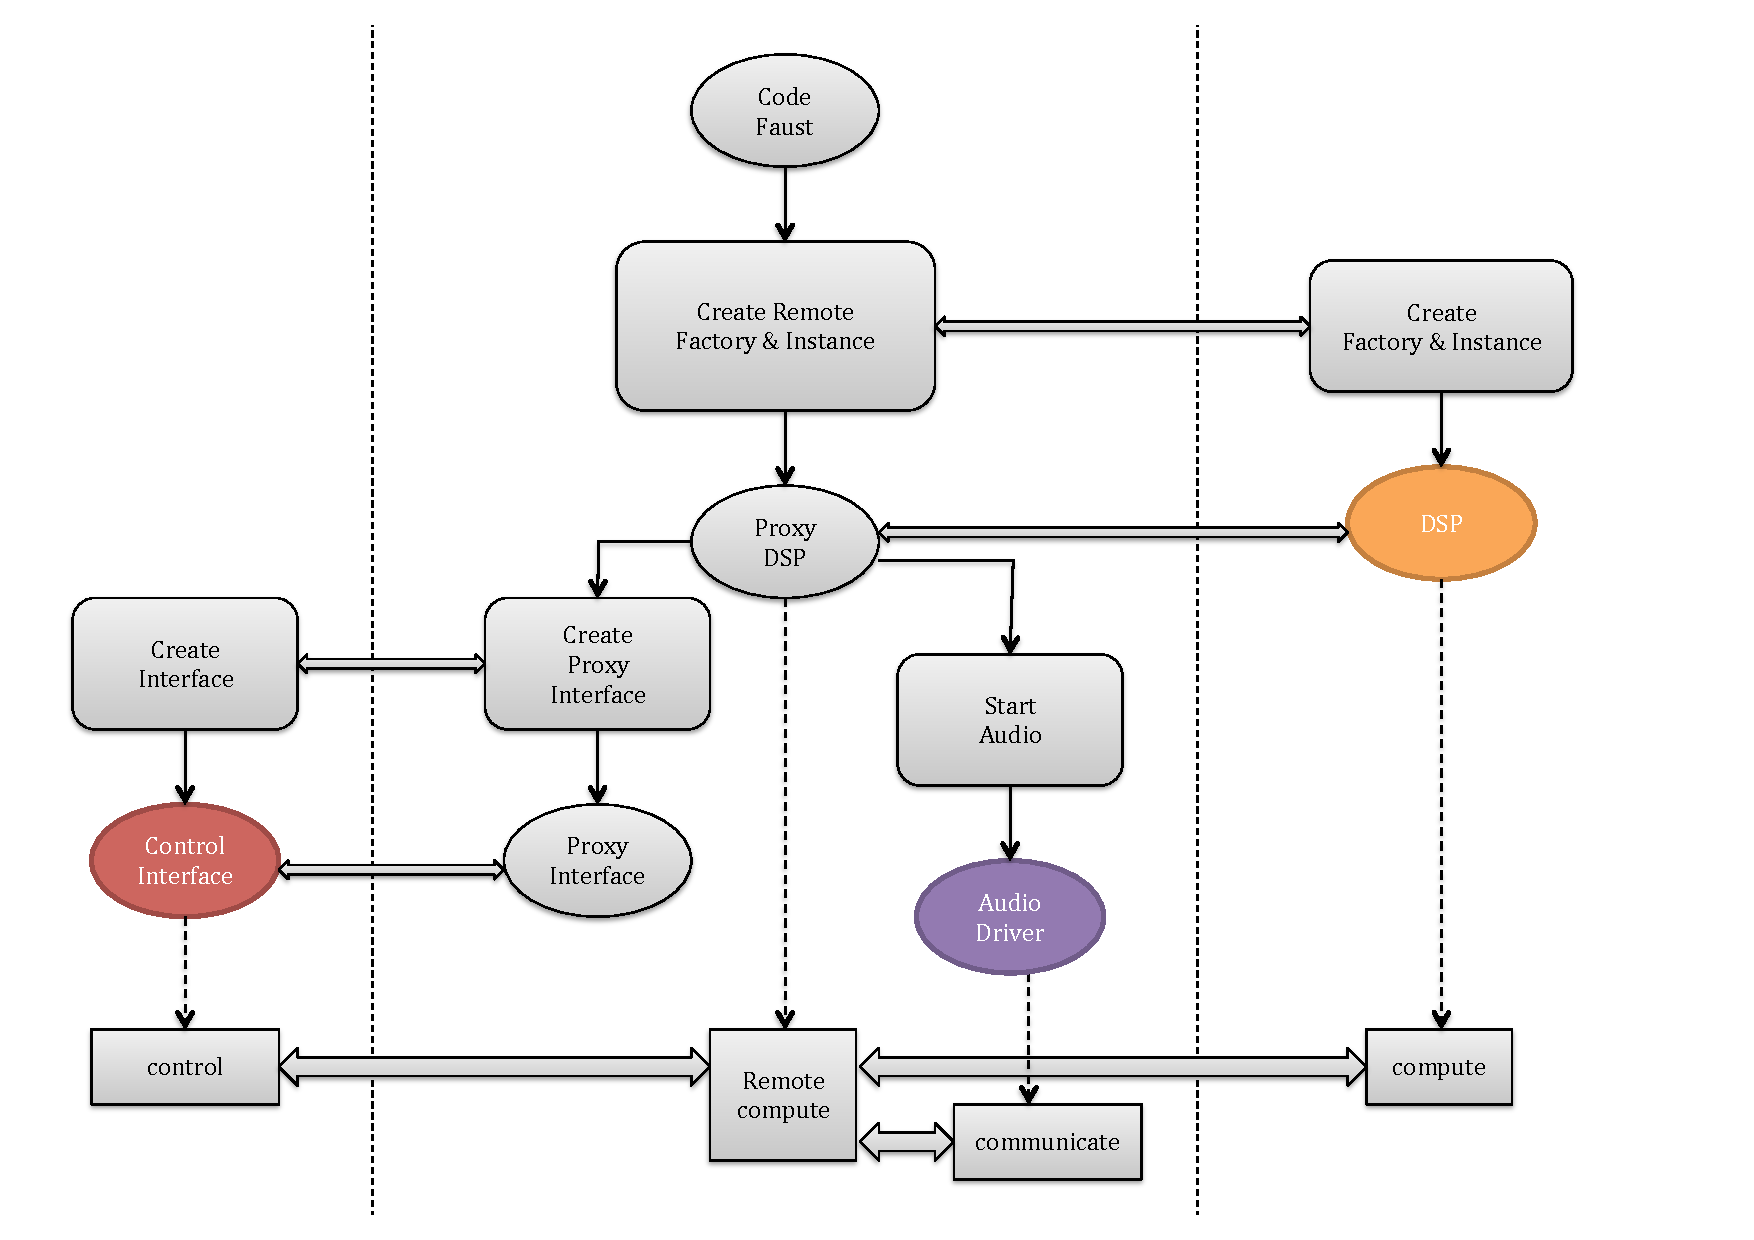
\includegraphics[width=\columnwidth]{images/CCC5}
\caption{Creation of the Interface/DSP/Driver for a remote processing and control}
\label{fig:CCC8}
\end{center}
\end{figure}

%%%%%%%%%%%%%%REMOTE CONTROL AND RENDERING ON MOBILE DEVICE%%%%%%%%%%%%%%%%%
\newpage
\subsection{ Control and audio on remote device}

This is the opposite of use case {\ref {remoteprocessing}}. \\

The mobile device discovers remote factories on FaustLive and requests a remote instance then has the control and communicate aspects over it. This use case is "more or less" available in FaustLive. The trick is to switch to a local remote processing server. The factory is then public on the server and accessible for remote devices. \\
An idea would be to have the possibility to "publish" the factory without quitting the local processing of the current running DSP. \\
Another important aspect is to have the possibility to synchronize the remote DSP with the FaustLive DSP. \\

The possibility to create the factory from the mobile device is represented on Figure 14, left part.

\begin{figure}[!h]
\begin{center}
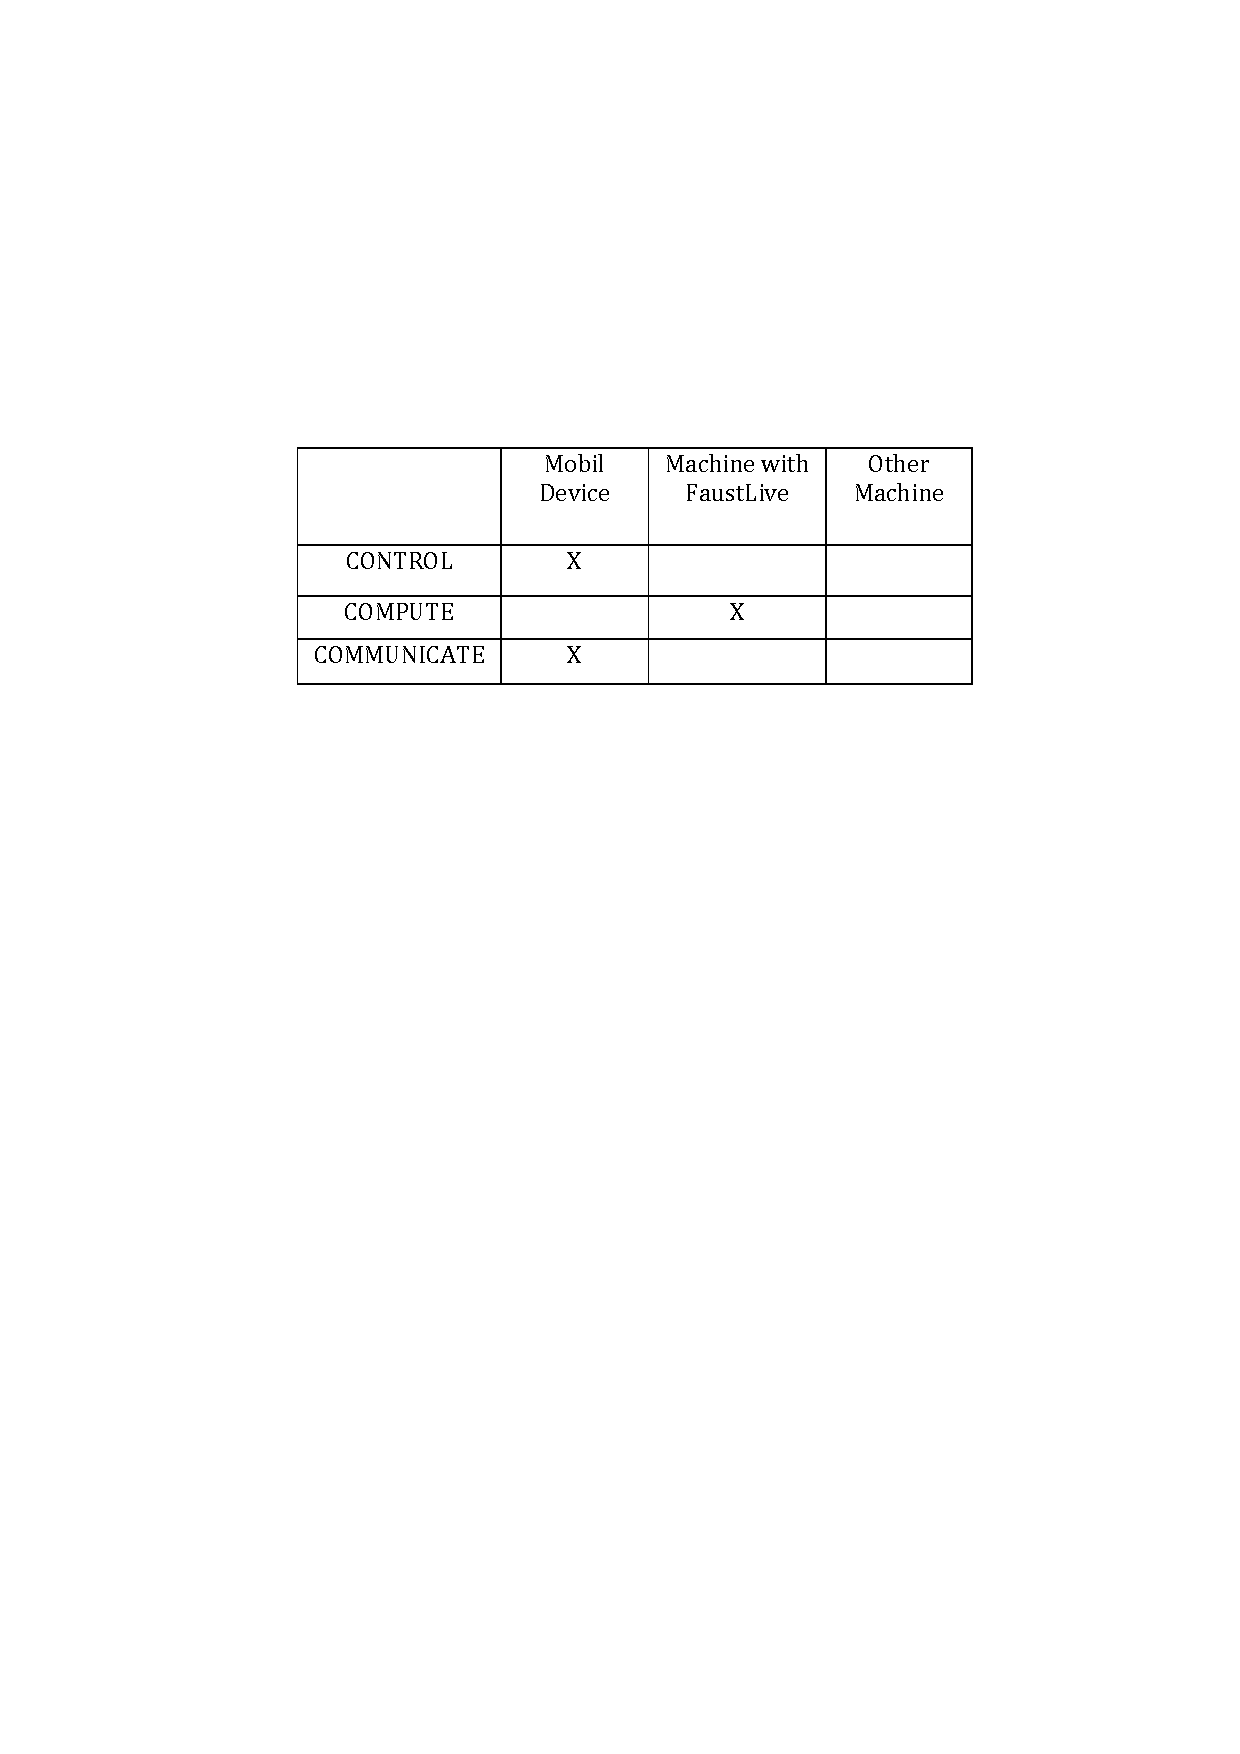
\includegraphics[width=0.7\columnwidth]{images/6CCC}
\caption{Control-Compute-Communicate Division with mobile device use case}
\label{fig:6CCC}
\end{center}
\end{figure}

\begin{figure}[!h]
\begin{center}
\begin{minipage}[c]{.45\linewidth}
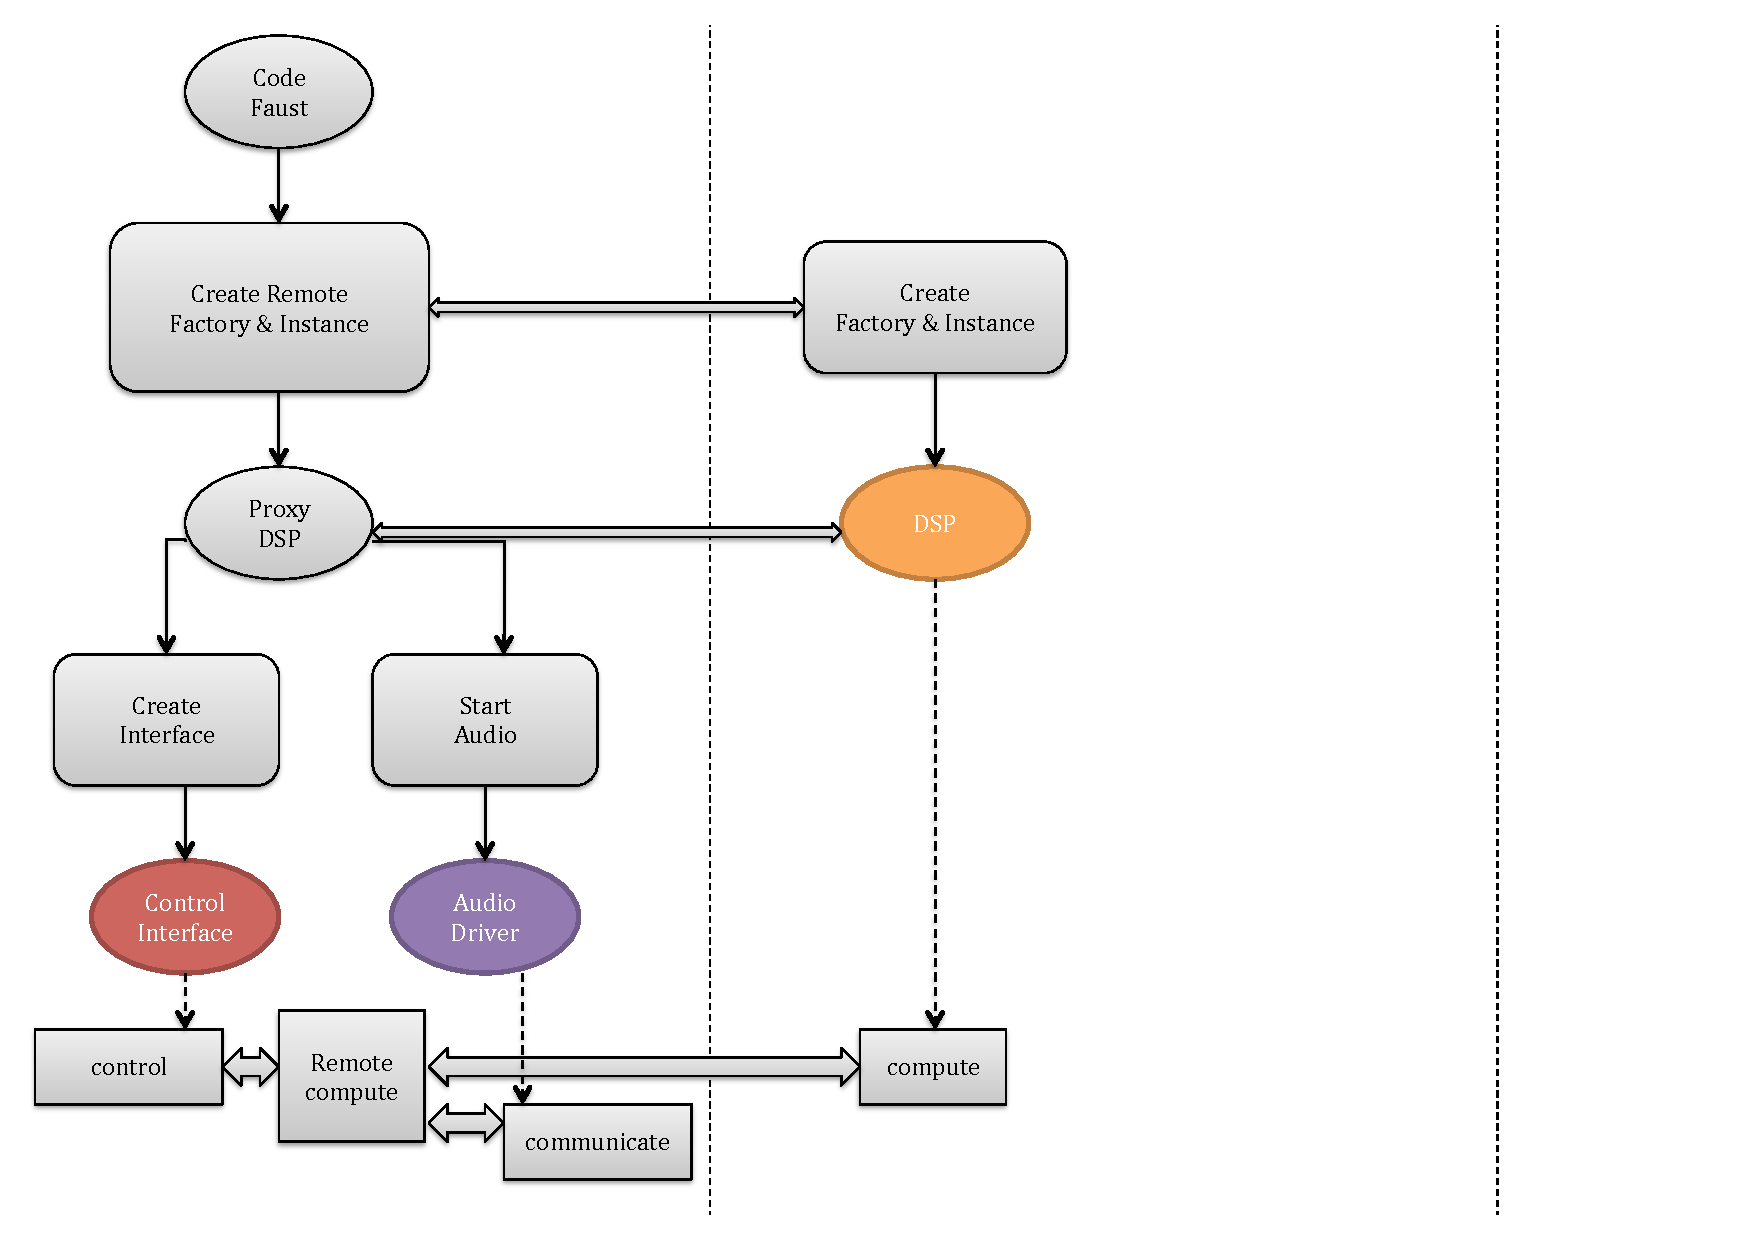
\includegraphics[width=\columnwidth]{images/CCC61}
\end{minipage}
\begin{minipage}[r]{.45\linewidth}
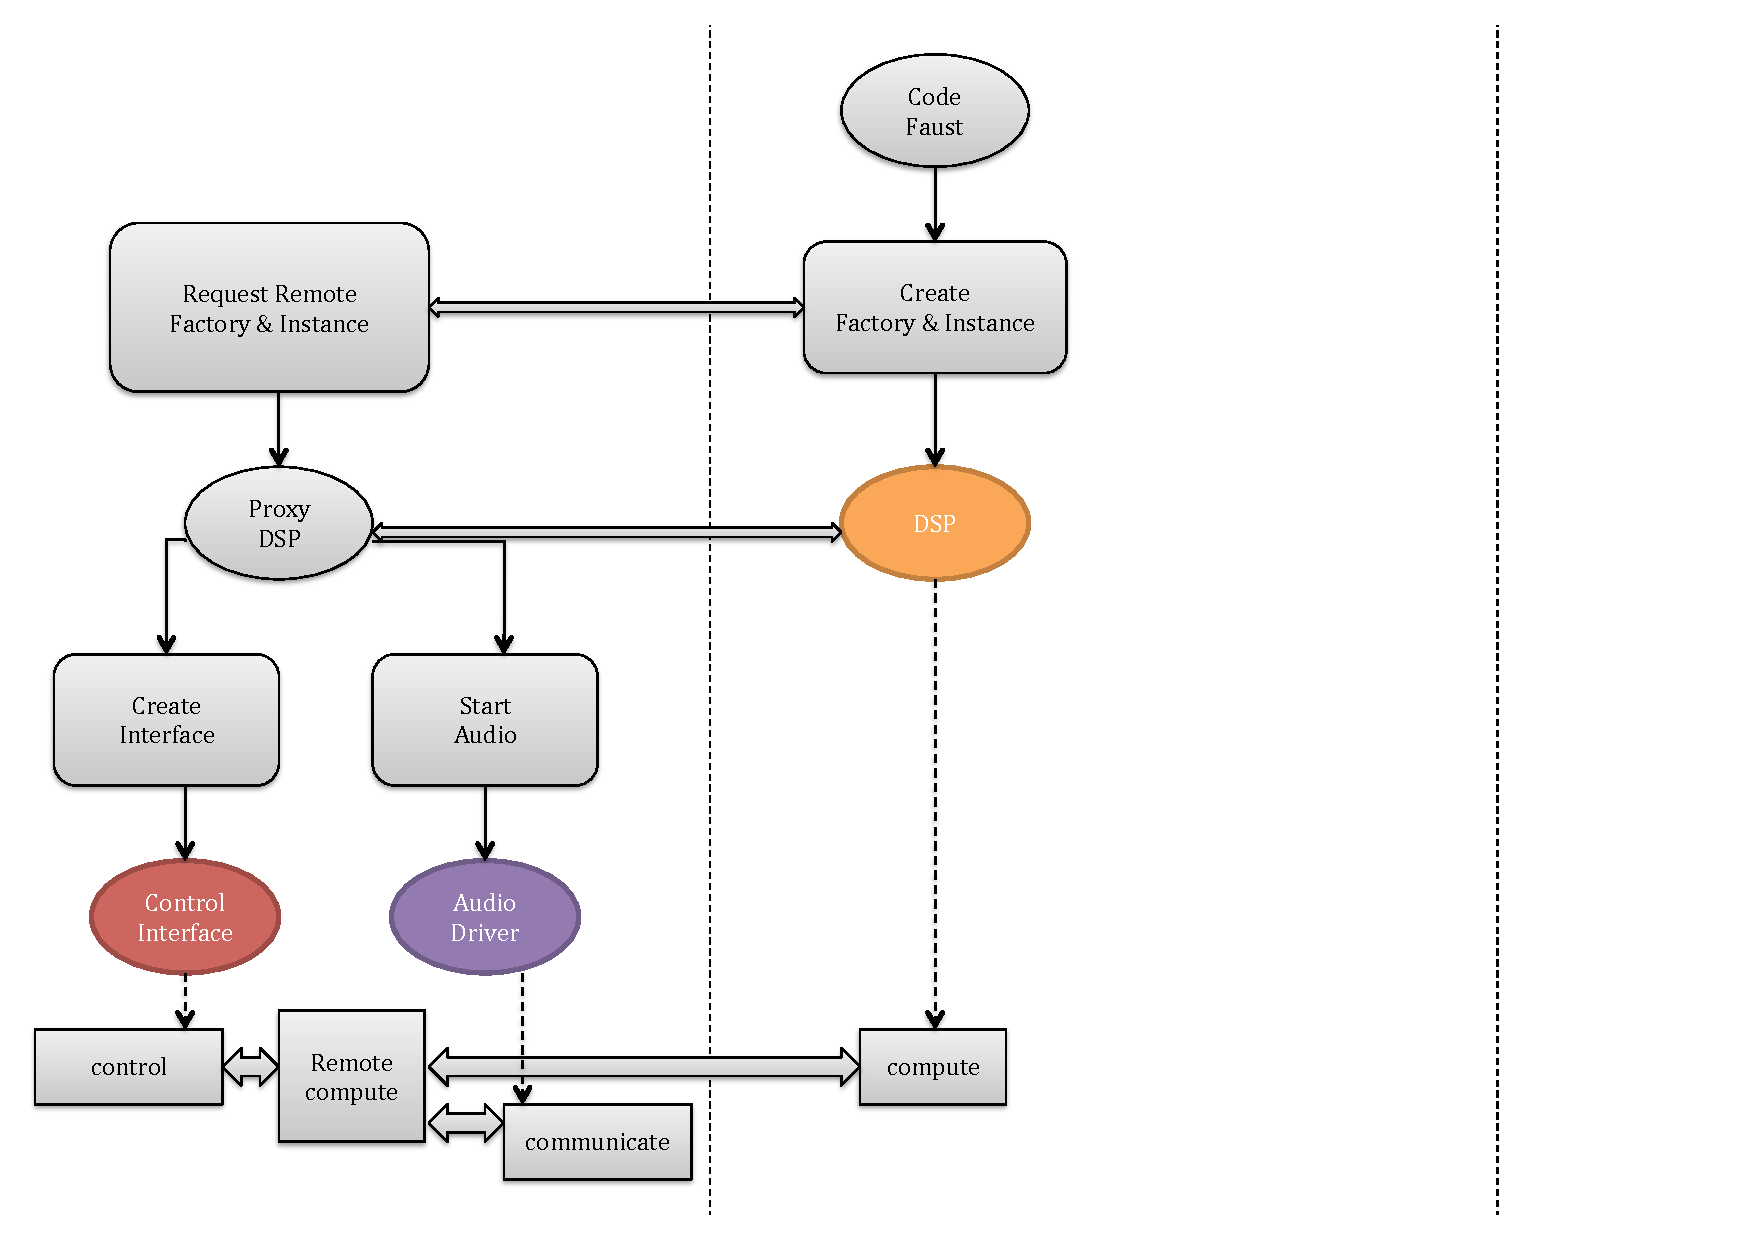
\includegraphics[width=\columnwidth]{images/CCC62}
\end{minipage}
\caption{Creation of the Interface/DSP/Driver for a remote control and rendering on a mobile device}
\label{fig:CCC4}
\end{center}
\end{figure}

%%%%%%%%%%%%%%REMOTE PROCESSING AND RENDERING%%%%%%%%%%%%%%%%%
\newpage
\subsection{ Remote processing and remote rendering}

The remote processing use cases are described on {\ref {remoteprocessing}}. \\

1 use case is implemented in FaustLive:
\begin{itemize}
\item NetJack is used to communicate between machines and render remotly. The communication between "Control" and "Communicate" runs through FaustLive. (combine \ref{remoterendering} and \ref{remoteprocessing})
\end{itemize}

The 2nd use case is conceivable but not implemented:
\begin{itemize}
\item The local driver (on the "Other Machine") is used to render. The communication between "Control" and "Communicate" does not run through FaustLive.
\end{itemize}

\begin{figure}[!h]
\begin{center}
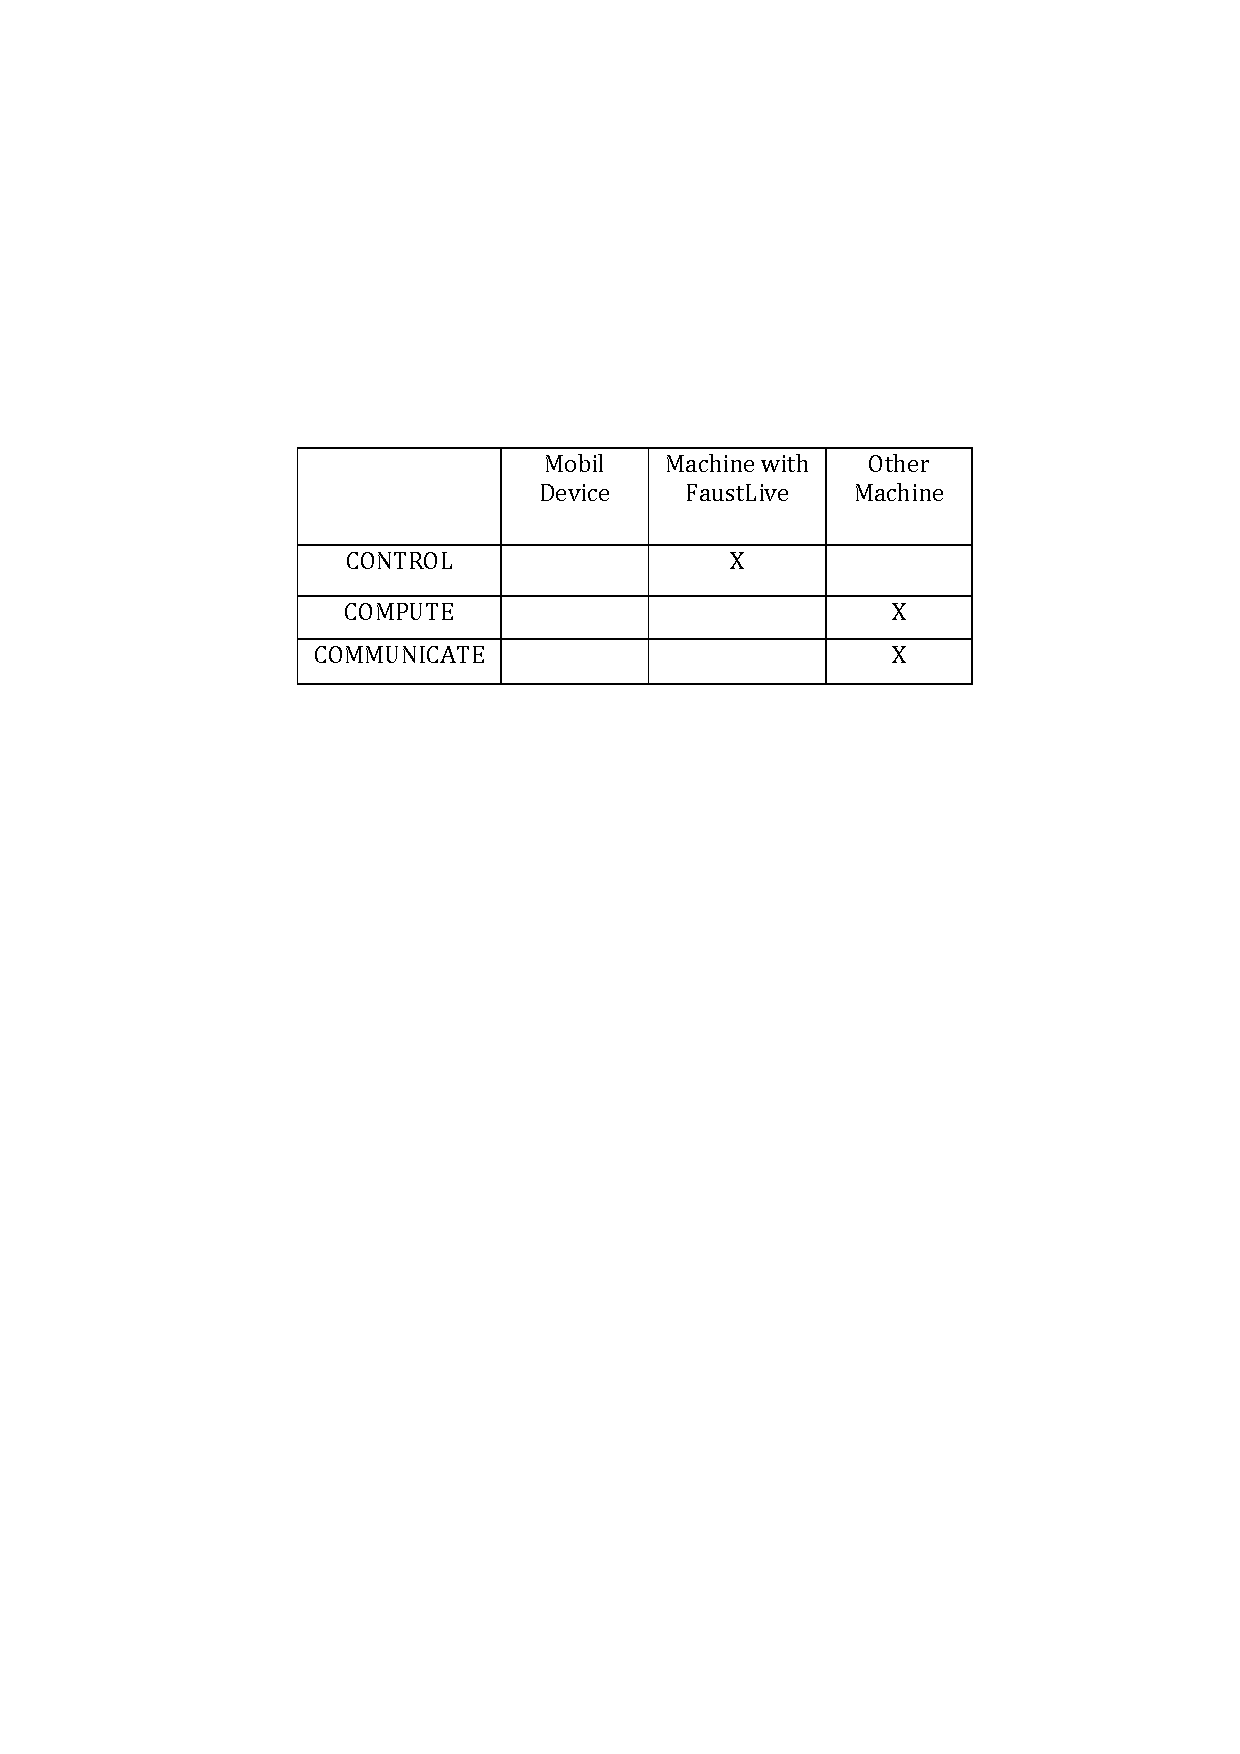
\includegraphics[width=0.7\columnwidth]{images/7CCC}
\caption{Control-Compute-Communicate Division with remote processing and remote audio rendering}
\label{fig:7CCC}
\end{center}
\end{figure}

\begin{figure}[!h]
\begin{center}
\begin{minipage}[c]{.45\linewidth}
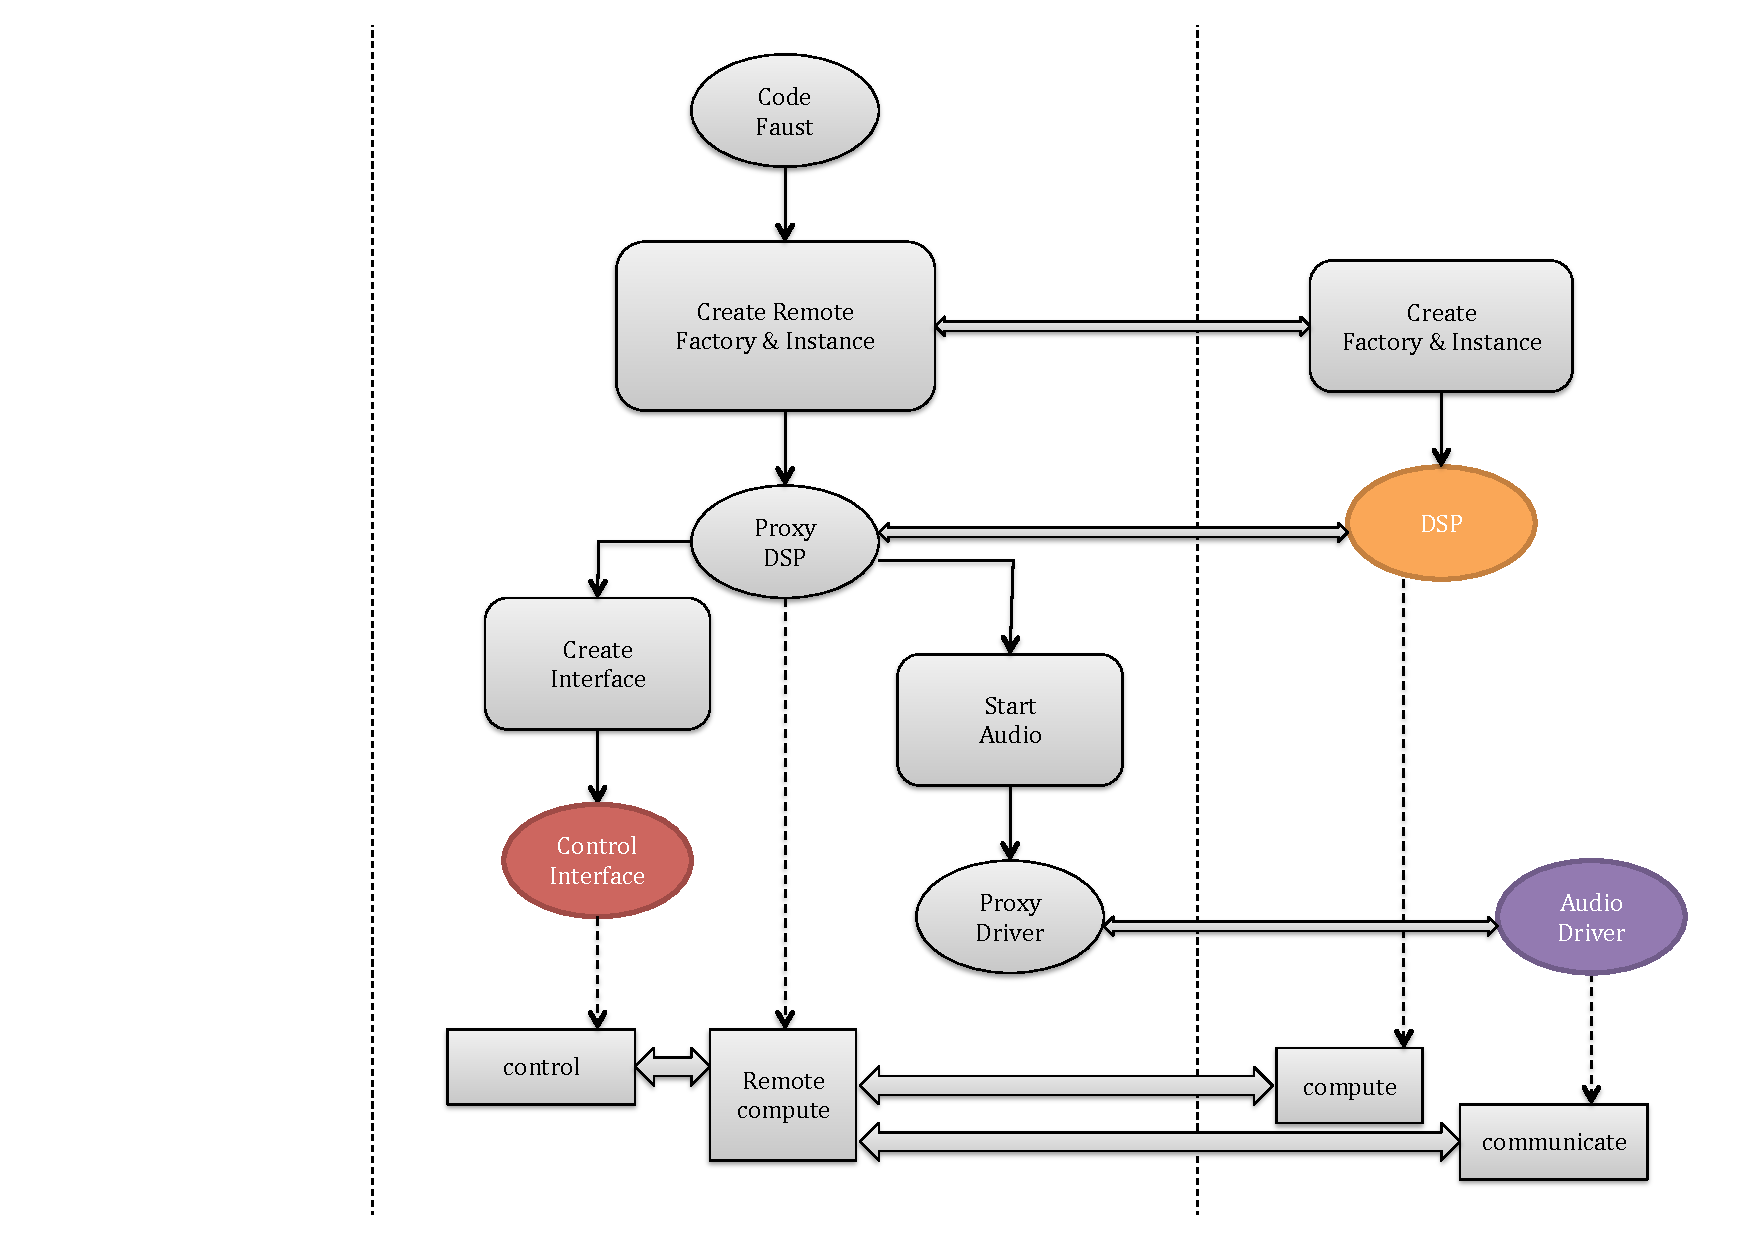
\includegraphics[width=\columnwidth]{images/CCC71}
\end{minipage}
\begin{minipage}[r]{.45\linewidth}
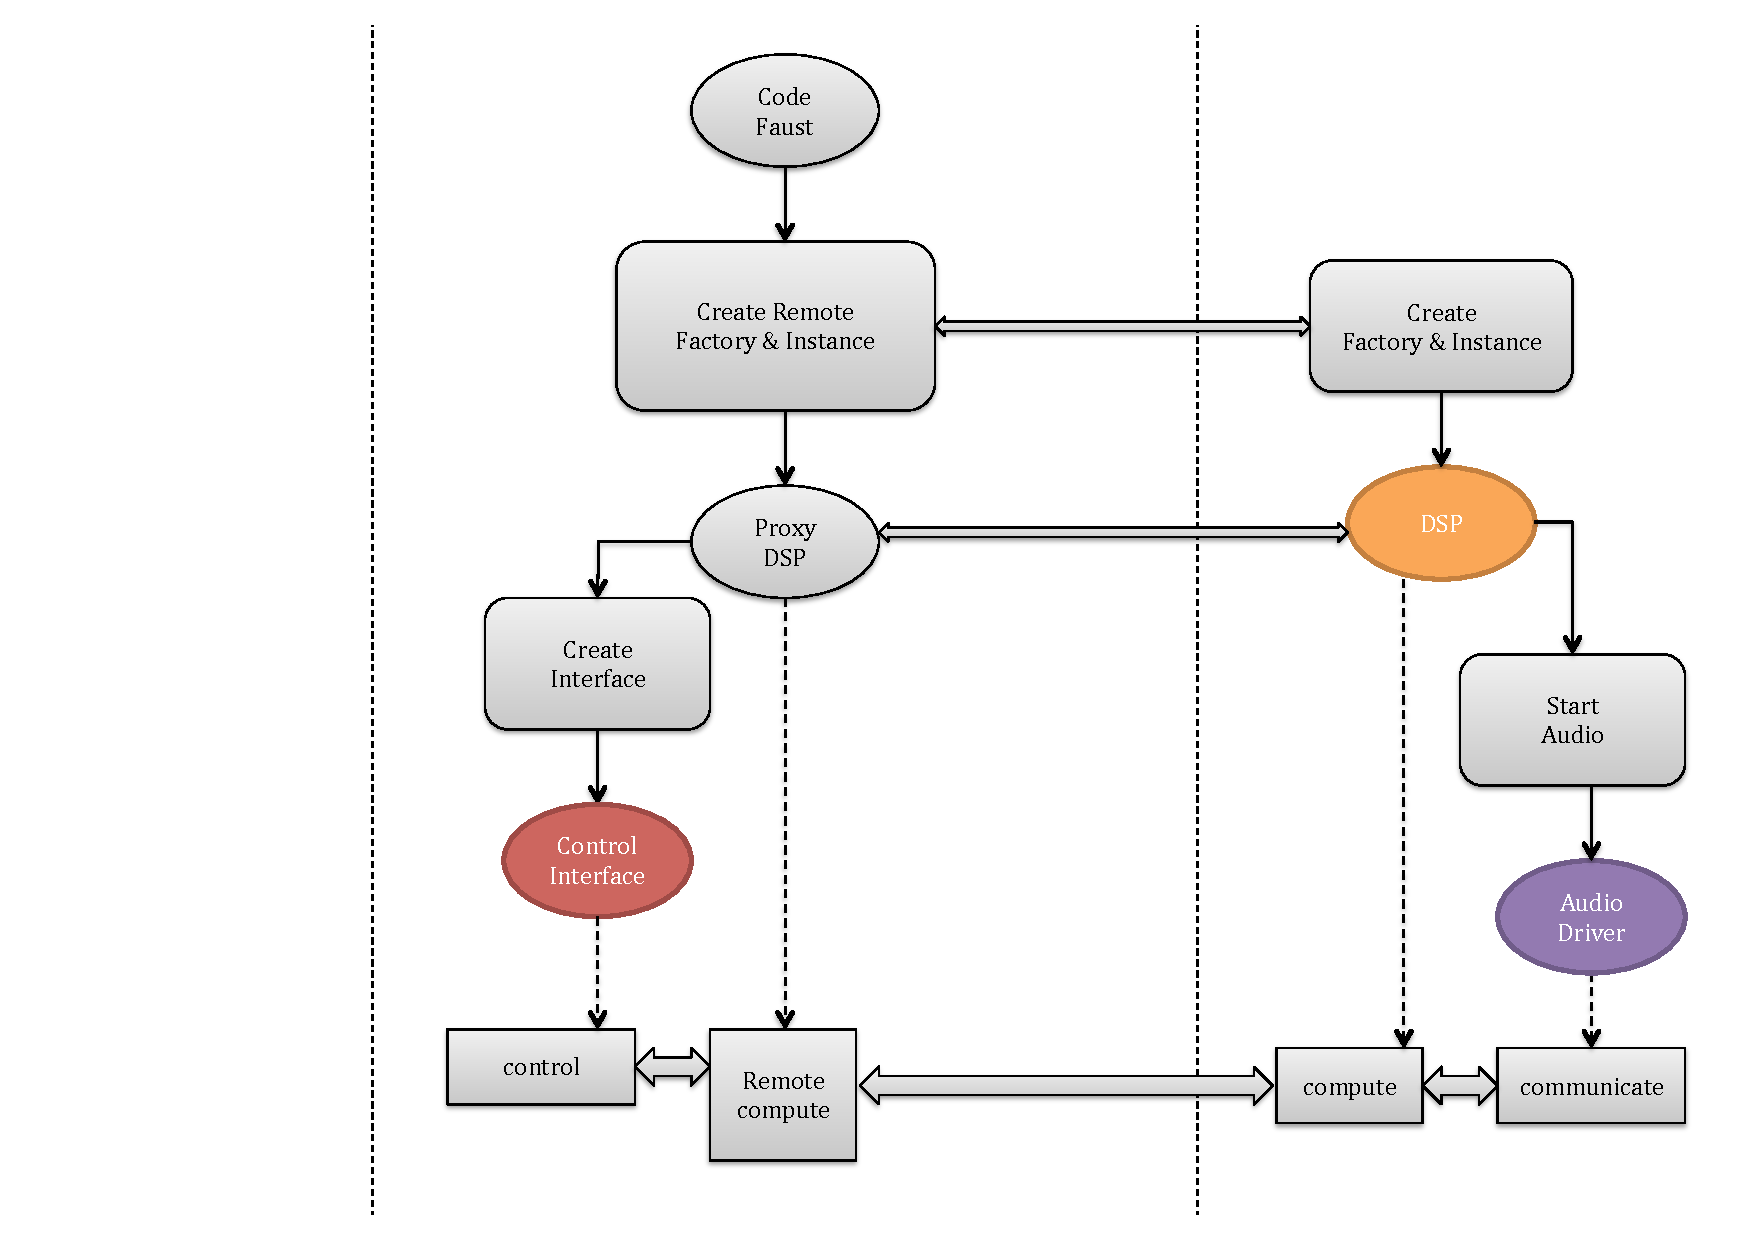
\includegraphics[width=\columnwidth]{images/CCC72}
\end{minipage}
\caption{Creation of the Interface/DSP/Driver for a remote processing and rendering use case}
\label{fig:CCC4}
\end{center}
\end{figure}

\end{document}




